\documentclass[a4paper,12pt,twoside]{memoir}

% Castellano
\usepackage[spanish,es-tabla]{babel}
\selectlanguage{spanish}
\usepackage[utf8]{inputenc}
\usepackage[T1]{fontenc}
\usepackage{lmodern} % Scalable font
\usepackage{microtype}
\usepackage{placeins}

\RequirePackage{booktabs}
\RequirePackage[table]{xcolor}
\RequirePackage{xtab}
\RequirePackage{multirow}

% Links
\usepackage[colorlinks]{hyperref}
\hypersetup{
  colorlinks,
  linkcolor={green!40!black},
  citecolor={blue!50!black},
  urlcolor={blue!80!black}
}

% Ecuaciones
\usepackage{amsmath}

% Rutas de fichero / paquete
\newcommand{\ruta}[1]{{\sffamily #1}}

% Párrafos
\nonzeroparskip


% Imagenes
\usepackage{graphicx}
\newcommand{\imagen}[2]{
	\begin{figure}[!h]
		\centering
		\includegraphics[width=0.9\textwidth]{#1}
		\caption{#2}\label{fig:#1}
	\end{figure}
	\FloatBarrier
}

\newcommand{\imagenflotante}[2]{
	\begin{figure}%[!h]
		\centering
		\includegraphics[width=0.9\textwidth]{#1}
		\caption{#2}\label{fig:#1}
	\end{figure}
}



% El comando \figura nos permite insertar figuras comodamente, y utilizando
% siempre el mismo formato. Los parametros son:
% 1 -> Porcentaje del ancho de página que ocupará la figura (de 0 a 1)
% 2 --> Fichero de la imagen
% 3 --> Texto a pie de imagen
% 4 --> Etiqueta (label) para referencias
% 5 --> Opciones que queramos pasarle al \includegraphics
% 6 --> Opciones de posicionamiento a pasarle a \begin{figure}
\newcommand{\figuraConPosicion}[6]{%
  \setlength{\anchoFloat}{#1\textwidth}%
  \addtolength{\anchoFloat}{-4\fboxsep}%
  \setlength{\anchoFigura}{\anchoFloat}%
  \begin{figure}[#6]
    \begin{center}%
      \Ovalbox{%
        \begin{minipage}{\anchoFloat}%
          \begin{center}%
            \includegraphics[width=\anchoFigura,#5]{#2}%
            \caption{#3}%
            \label{#4}%
          \end{center}%
        \end{minipage}
      }%
    \end{center}%
  \end{figure}%
}

%
% Comando para incluir imágenes en formato apaisado (sin marco).
\newcommand{\figuraApaisadaSinMarco}[5]{%
  \begin{figure}%
    \begin{center}%
    \includegraphics[angle=90,height=#1\textheight,#5]{#2}%
    \caption{#3}%
    \label{#4}%
    \end{center}%
  \end{figure}%
}
% Para las tablas
\newcommand{\otoprule}{\midrule [\heavyrulewidth]}
%
% Nuevo comando para tablas pequeñas (menos de una página).
\newcommand{\tablaSmall}[5]{%
 \begin{table}
  \begin{center}
   \rowcolors {2}{gray!35}{}
   \begin{tabular}{#2}
    \toprule
    #4
    \otoprule
    #5
    \bottomrule
   \end{tabular}
   \caption{#1}
   \label{tabla:#3}
  \end{center}
 \end{table}
}

%
% Nuevo comando para tablas pequeñas (menos de una página).
\newcommand{\tablaSmallSinColores}[5]{%
 \begin{table}[H]
  \begin{center}
   \begin{tabular}{#2}
    \toprule
    #4
    \otoprule
    #5
    \bottomrule
   \end{tabular}
   \caption{#1}
   \label{tabla:#3}
  \end{center}
 \end{table}
}

\newcommand{\tablaApaisadaSmall}[5]{%
\begin{landscape}
  \begin{table}
   \begin{center}
    \rowcolors {2}{gray!35}{}
    \begin{tabular}{#2}
     \toprule
     #4
     \otoprule
     #5
     \bottomrule
    \end{tabular}
    \caption{#1}
    \label{tabla:#3}
   \end{center}
  \end{table}
\end{landscape}
}

%
% Nuevo comando para tablas grandes con cabecera y filas alternas coloreadas en gris.
\newcommand{\tabla}[6]{%
  \begin{center}
    \tablefirsthead{
      \toprule
      #5
      \otoprule
    }
    \tablehead{
      \multicolumn{#3}{l}{\small\sl continúa desde la página anterior}\\
      \toprule
      #5
      \otoprule
    }
    \tabletail{
      \hline
      \multicolumn{#3}{r}{\small\sl continúa en la página siguiente}\\
    }
    \tablelasttail{
      \hline
    }
    \bottomcaption{#1}
    \rowcolors {2}{gray!35}{}
    \begin{xtabular}{#2}
      #6
      \bottomrule
    \end{xtabular}
    \label{tabla:#4}
  \end{center}
}

%
% Nuevo comando para tablas grandes con cabecera.
\newcommand{\tablaSinColores}[6]{%
  \begin{center}
    \tablefirsthead{
      \toprule
      #5
      \otoprule
    }
    \tablehead{
      \multicolumn{#3}{l}{\small\sl continúa desde la página anterior}\\
      \toprule
      #5
      \otoprule
    }
    \tabletail{
      \hline
      \multicolumn{#3}{r}{\small\sl continúa en la página siguiente}\\
    }
    \tablelasttail{
      \hline
    }
    \bottomcaption{#1}
    \begin{xtabular}{#2}
      #6
      \bottomrule
    \end{xtabular}
    \label{tabla:#4}
  \end{center}
}

%
% Nuevo comando para tablas grandes sin cabecera.
\newcommand{\tablaSinCabecera}[5]{%
  \begin{center}
    \tablefirsthead{
      \toprule
    }
    \tablehead{
      \multicolumn{#3}{l}{\small\sl continúa desde la página anterior}\\
      \hline
    }
    \tabletail{
      \hline
      \multicolumn{#3}{r}{\small\sl continúa en la página siguiente}\\
    }
    \tablelasttail{
      \hline
    }
    \bottomcaption{#1}
  \begin{xtabular}{#2}
    #5
   \bottomrule
  \end{xtabular}
  \label{tabla:#4}
  \end{center}
}



\definecolor{cgoLight}{HTML}{EEEEEE}
\definecolor{cgoExtralight}{HTML}{FFFFFF}

%
% Nuevo comando para tablas grandes sin cabecera.
\newcommand{\tablaSinCabeceraConBandas}[5]{%
  \begin{center}
    \tablefirsthead{
      \toprule
    }
    \tablehead{
      \multicolumn{#3}{l}{\small\sl continúa desde la página anterior}\\
      \hline
    }
    \tabletail{
      \hline
      \multicolumn{#3}{r}{\small\sl continúa en la página siguiente}\\
    }
    \tablelasttail{
      \hline
    }
    \bottomcaption{#1}
    \rowcolors[]{1}{cgoExtralight}{cgoLight}

  \begin{xtabular}{#2}
    #5
   \bottomrule
  \end{xtabular}
  \label{tabla:#4}
  \end{center}
}


















\graphicspath{ {./img/} }

% Capítulos
\chapterstyle{bianchi}
\newcommand{\capitulo}[2]{
	\setcounter{chapter}{#1}
	\setcounter{section}{0}
	\chapter*{#2}
	\addcontentsline{toc}{chapter}{#2}
	\markboth{#2}{#2}
}

% Apéndices
\renewcommand{\appendixname}{Apéndice}
\renewcommand*\cftappendixname{\appendixname}

\newcommand{\apendice}[1]{
	%\renewcommand{\thechapter}{A}
	\chapter{#1}
}

\renewcommand*\cftappendixname{\appendixname\ }

% Formato de portada
\makeatletter
\usepackage{xcolor}
\newcommand{\tutor}[1]{\def\@tutor{#1}}
\newcommand{\course}[1]{\def\@course{#1}}
\definecolor{cpardoBox}{HTML}{E6E6FF}
\def\maketitle{
  \null
  \thispagestyle{empty}
  % Cabecera ----------------
\noindent
\includegraphics[width=\textwidth]{cabecera}\vspace{1cm}%
  \vfill
  % Título proyecto y escudo informática ----------------
  \colorbox{cpardoBox}{%
    \begin{minipage}{.8\textwidth}
      \vspace{.5cm}\Large
      \begin{center}
      \textbf{TFG del Grado en Ingeniería Informática}\vspace{.6cm}\\
      \textbf{\LARGE\@title{}}
      \end{center}
      \vspace{.2cm}
    \end{minipage}

  }%
  \hfill\begin{minipage}{.20\textwidth}
    
\includegraphics[width=\textwidth]{escudoInfor}
  \end{minipage}
  \vfill
  % Datos de alumno, curso y tutores ------------------
  \begin{center}%
  {%
    \noindent\LARGE
    Presentado por \\ \@author{}\\ 
    en la Universidad de Burgos --- \@date{}\\
    Tutores: \@tutor{}\\
  }%
  \end{center}%
  \null
  \cleardoublepage
  }
\makeatother

\newcommand{\nombre}{José Eduardo Risco Sánchez-Cortés} %%% cambio de comando

% Datos de portada
\title{{\Huge SurveyingPointCode}\\[0.5cm]Automatización del proceso de delineación a partir de datos de un Levantamiento Topográfico.}
\author{\nombre}
\tutor{Dr. César García-Osorio\\ y Dr. Carlos López Nozal}
\date{\today}

\begin{document}

\maketitle





%%%%%%%%%%%%%%%%%%%%%%%%%%%%%%%%%%%%%%%%%%%%%%%%%%%%%%%%%%%%%%%%%%%%%%%%%%%%%%%%%%%%%%%%
\thispagestyle{empty}


\noindent
\includegraphics[width=\textwidth]{cabecera}\vspace{1cm}

\noindent D. César García-Osorio y D. Carlos López Nozal, profesores del departamento de Ingeniería Civil, área de Lenguajes y Sistemas Informáticos.

\noindent Exponen:\\
\noindent Que el alumno D. \nombre, con DNI 40441256B , ha realizado el Trabajo final de Grado en Ingeniería Informática titulado:\\
\noindent "SurveyingPointCode - Automatización del proceso de delineación a partir de datos de un Levantamiento Topográfico"

\noindent Y que dicho trabajo ha sido realizado por el alumno bajo la dirección del que suscribe, en virtud de lo cual se autoriza su presentación y defensa.

\begin{center} %\large
En Burgos, {\large \today}
\end{center}

\vfill\vfill\vfill

% Author and supervisor
\begin{minipage}{0.45\textwidth}
\begin{flushleft} %\large
Vº. Bº. del Tutor:\\[2cm]
D. César García-Osorio
\end{flushleft}
\end{minipage}
\hfill
\begin{minipage}{0.45\textwidth}
\begin{flushleft} %\large
Vº. Bº. del tutor:\\[2cm]
D. Carlos López Nozal
\end{flushleft}
\end{minipage}
\hfill

\vfill

% para casos con solo un tutor comentar lo anterior
% y descomentar lo siguiente
%Vº. Bº. del Tutor:\\[2cm]
%D. nombre tutor





\frontmatter

% Abstract en castellano
\renewcommand*\abstractname{Resumen}
\begin{abstract}
En el campo de la Topografía, hay trabajos cuyo objetivo es obtener el plano de un levantamiento topográfico. Este trabajo se divide en dos partes, trabajo de campo y delineación. Es importante entender que la relación entre las dos partes es fundamental para poder reducir al máximo los recursos invertidos tanto en la parte del trabajo de campo como en la de delineación. 

Con este trabajo, se pretende que mediante una codificación definida por el usuario en el trabajo de campo, (para cada punto medido), se optimice la medición en campo y posteriormente, la codificación permita la generación automática del plano final, en un archivo de \textbf{CAD} (con formato \textbf {DXF}), teniendo en cuenta la distribución de los puntos en diferentes capas, generación de líneas, curvas, simbología, etc.

Con este propósito se ha desarrollado la aplicación SurveyingPointCode, aplicación Web que realiza la conversión de un archivo que contiene los datos de un levantamiento topográfico a un archivo \textbf {DXF}.

\end{abstract}

\renewcommand*\abstractname{Descriptores}
\begin{abstract}
Levantamiento topográfico, CAD, DXF, código punto, delineación, aplicación Web. 
\end{abstract}

\clearpage

% Abstract en inglés
\renewcommand*\abstractname{Abstract}
\begin{abstract}
In the field of Topography, there are projects whose objective is to obtain the plan of a topographic survey. This project is divided in two parts; survey work and delineation. It is important to understand that the relationship between these two parts will be fundamental to be able to reduce to the maximum the resources invested in both the survey work and the delineation work.

The main purpose of this work is to optimize the data collection through a coding defined by the user in the field work (for each measured point). Subsequently the coding will allow the automatic generation of the final plan, in a \textbf{CAD} file. (with \textbf {DXF} format), taking into account the distribution of points in different layers, generation of lines, curves, symbology, etc.

For this purpose, the SurveyingPointCode application has been developed, a Web application that performs the conversion of a file that contains the data from a topographic survey to a \textbf {DXF} file

\end{abstract}

\renewcommand*\abstractname{Keywords}
\begin{abstract}
Topographical survey, CAD, DXF, point code, delineation, Web application.
\end{abstract}
\clearpage
% Indices
\tableofcontents
\clearpage
\listoffigures
\clearpage
\listoftables
\clearpage
\mainmatter
\capitulo{1}{Introducción}
\section{Introducción}
Uno de los trabajos que se realiza habitualmente en el campo de la Topografía y Cartografía, es la representación en un plano de los datos obtenidos en un levantamiento topográfico. Pongamos como ejemplo que se nos pide como producto final, un plano basado en un levantamiento topográfico de una zona de una ciudad para realizar el estudio de unas futuras obras. El plano debe contener todos los elementos existentes que sean de interés para este estudio, como, por ejemplo: edificios, aceras, viales, redes de saneamiento, abastecimiento, eléctricas, mobiliario urbano, etc.

Este trabajo se realizará en dos fases; la primera, el trabajo de campo, donde se realiza el levantamiento topográfico, adquisición de datos, que consiste en la medición georreferenciada de todos los elementos que sean de interés y que deben aparecer en el plano. La segunda fase es la de delineación, en la que se ‘dibuja’ el plano. Hay que aclarar que, en la fase del levantamiento topográfico, solo se miden puntos, y es en la fase de delineación donde tenemos que crear todos los elementos, como líneas, curvas, símbolos, etc   

Un problema importante al que nos enfrentamos es la gran cantidad de tiempo y recursos que invertimos en gestionar los datos obtenidos en campo para obtener un plano, alargando en exceso el desarrollo y entrega de un proyecto.
Con este planteamiento surge la necesidad de crear una aplicación que consiga automatizar este trabajo el máximo posible y así obtener un ahorro de tiempo y de recursos, fundamental en nuestros proyectos.
Puede parecer a priori un trabajo sencillo y rápido de realizar, con una herramienta de CAD, uniendo puntos manualmente para crear líneas, u otros elementos, claro está, si tienes un levantamiento topográfico con 30 puntos y recuerdas como lo has hecho en campo, pero cuando tienes un levantamiento con 1000 puntos, e intervienen varias personas en él, se puede convertir en un trabajo muy complicado e insufrible de realizar.
Una herramienta así no existe mercado, algunos programas como AutoCAD disponen de algún módulo a mayores del programa, que permiten hacer algo similar, pero con un resultado muy pobre respecto a lo que aquí se plantea.

La principal ventaja que aporta el uso de esta aplicación es el importante ahorro de tiempo y recursos que obtenemos en la realización de un trabajo. Por ejemplo, un trabajo de campo con 1000 puntos, con una codificación compleja, es decir con múltiples y diferentes elementos, una persona con habilidad en manejo de aplicaciones CAD, puede invertir alrededor de 2 horas. Esta aplicación pretende que ese proceso sea automático e inmediato. No debemos olvidar que el uso de una codificación totalmente aleatoria por el usuario a la hora de realizar el trabajo de campo también va a permitir obtener un importante ahorro de recursos, en esa parte del trabajo.
Otras ventajas son:
\begin{itemize}
	\item Es una aplicación web, por lo que los usuarios no necesitan instalar nada en sus equipos y pueden acceder desde cualquier lugar.
	\item Facilidad de uso, no hacen falta conocimientos técnicos en el uso de herramientas CAD.
\end{itemize}
\section{Contenido del proyecto}

La estructura de la memoria es la siguiente:

\begin{itemize}
	\item \textbf {Introducción:} breve descripción del contenido del trabajo y de la estructura de la memoria.
	\item \textbf {Objetivos del proyecto:} objetivos que se persiguen con la realización del proyecto.
	\item \textbf {Conceptos teóricos:} breve explicación de los conceptos necesarios para el desarrollo de la solución propuesta.
	\item \textbf {Técnicas y herramientas:} presentación de las técnicas metodológicas y las herramientas de desarrollo que se han utilizado para llevar a cabo el proyecto.
	\item \textbf {Aspectos relevantes del desarrollo:} descripción de los aspectos más importantes ocurridos a lo largo del desarrollo del proyecto.
	\item \textbf {Trabajos relacionados:} pequeño resumen de los trabajos y proyectos ya realizados en el campo del proyecto en curso.
	\item \textbf {Conclusiones y líneas de trabajo futuras:} resumen acerca de los conocimientos adquiridos y posibles aspectos de mejora o expansión de la solución aportada.
\end{itemize}

Además, se han desarrollado los siguientes anexos:

\begin{itemize}
	\item \textbf {Plan de Proyecto Software:} explicación sobre la planificación temporal llevada a cabo, así como un estudio de viabilidad del proyecto.
	\item \textbf {Especificación de requisitos:} descripción de la fase de análisis de la aplicación.
	\item \textbf {Especificación de diseño:} explicación y descripción del diseño de la aplicación.
	\item \textbf {Documentación técnica de programación:} recoge los aspectos más relevantes relacionados con el código fuente (estructura, compilación, instalación, ejecución, pruebas, etc.).
	\item \textbf {Documentación de usuario:} manual de usuario que permita conocer el funcionamiento la aplicación.
\end{itemize}

Por último, hay que indicar que el proyecto se encuentra disponible en el siguiente enlace:\\
 \url{https://github.com/EduardoRisco/SurveyingPointCode}
\clearpage
\capitulo{2}{Objetivos del proyecto}

A continuación, se detallan los diferentes objetivos que han motivado la realización del proyecto.
\section{Objetivos generales}
\begin{itemize}

	\item Desarrollar una aplicación web que permita obtener un archivo DXF a partir de los datos de un levantamiento topográfico.

	\item Definir un tipo de codificación para los puntos medidos en campo, que sea interpretada por la aplicación, automatice el proceso de dibujo y mejore el rendimiento en el trabajo de campo.

	\item Permitir al usuario crear una cuenta.

	\item Permitir al usuario subir :  archivos de campo, archivos de configuración personalizados de la transformación y archivos DXF, con símbolos creados por el usuario.

	\item Permitir al usuario modificar o elegir, en la interfaz, los nombres de las capas de CAD, colores y símbolos existentes, y asociarlos a los códigos de campo

	\item Permitir al usuario elegir la versión de CAD para generar el archivo DXF.

	\item Permitir al usuario almacenar en su equipo, el archivo DXF generado.
\end{itemize}
\section{Objetivos técnicos}

\begin{itemize}
\item Desarrollar una aplicación web utilizando el framework \textbf {Flask}.

\item Utilizar \textbf {PLY}\footnote{\textsl{PLY}: \url{https://pypi.org/project/ply/}}   (Python Lex-Yacc), como analizador sintáctico, para reconocer la validez de los archivos de entrada.

\item Utilizar \textbf {ezdxf}\footnote{\textsl{ezdf}: \url{https://ezdxf.readthedocs.io/en/latest/index.html}}  ,  para leer, modificar y crear archivos DXF. 

\item Utilizar \textbf {Bootstrap}, para crear el sitio web.

\item Utilizar \textbf {TinyColor}\footnote{\textsl{TinyColor}: \url{https://github.com/bgrins/TinyColor}} para poder definir los colores con los estándares de AutoCAD.

\item Utilizar  \textbf {PostGIS}\footnote{\textsl{PostGIS}: \url{https://postgis.net/}} como sistema de base de datos.

\item Realizar test unitarios.

\item Hacer uso de la herramienta \textbf {CODEBEAT} para comprobar la calidad del código.

\item Desplegar la aplicación usando \textbf {Docker} .

\item Utilizar \textbf {Git} como sistema de control de versiones distribuido junto con la plataforma \textbf {GitHub}.

\item Aplicar la metodología ágil \textbf {Scrum} para el desarrollo del software.

\item Utilizar \textbf {ZenHub} como herramienta de gestión de proyectos.
\end{itemize}

\section{Objetivos personales}
\begin{itemize}
\item Mejorar los recursos invertidos y facilitar el trabajo, a la hora de realizar un levantamiento topográfico.

\item Realizar el proyecto como un trabajo real, aplicando los conocimientos adquiridos en la realización del Grado.

\item Utilizar herramientas y metodologías demandadas en el mercado laboral; Git, desarrollo Web, Docker, etc.
\end{itemize}
\capitulo{3}{Conceptos teóricos}

En este apartado se explican conceptos los básicos necesarios para entender el contexto en que se desarrolla este proyecto, respecto a lo que aquí se pretende, haciendo hincapié en la topografía y el dibujo en CAD. 

\section{Levantamiento topográfico}

Un levantamiento topográfico consiste en la medición de distintos puntos, mediante cálculos topográficos, donde se obtienen las coordenadas de estos, generalmente las coordenadas $X$, $Y$ y $Z$. Estas coordenadas nos indican su posición exacta en el espacio. 

El software que tienen los equipos de topografía; como teodolitos, estaciones totales o GPS, permiten asociar a cada punto un texto en el momento de medir el punto y así, el punto queda registrado con ese campo.

Este campo de texto, que de aquí en adelante llamaremos código de punto, es el elemento en el que se centra este proyecto. El algoritmo diseñado debe saber interpretar este código de punto. Como veremos más adelante, este nos puede indicar una o múltiples cosas a la vez, lo que conlleva mayor dificultad a la hora de definir el formato que debe tener este. Tiene que aportar la máxima información posible, pero a la vez tiene que ser muy sencillo en su estructura y de una longitud lo más corta posible. No es muy viable tener que estar mucho tiempo tecleando, ya que se perdería mucho tiempo y alargaría en exceso el trabajo de campo.

\section{Archivo DXF---Elementos del dibujo}

DXF (acrónimo del inglés \emph{Drawing Exchange Format}) es un formato de archivo para dibujos de diseño asistido por computadora, creado por \emph{AutoCAD}. Formato muy extendido y utilizado por la mayoría de programas de CAD, como por ejemplo: \emph{AutoCAD, MicroStation, FreeCAD, DraftSight},... y también por programas de GIS, como: \emph{ArcGIS, QGIS, gvSIG}, ...

Para entender de forma sencilla los elementos de los que está compuesto un archivo DXF, solo se tratarán aquellos elementos que se utilizan en esta aplicación, de otra forma, la explicación sería muy extensa.
Simplificando, se procede a hacer una diferenciación entre los elementos que queremos dibujar, que llamaremos elementos gráficos, y los elementos no gráficos.

\textbf {Elementos gráficos}
\begin{itemize}
\item\textbf{Puntos:} En este caso es el elemento básico, ya que en una medición topográfica solo se obtienen puntos. El resto de los elementos que se exponen a continuación están basados en la posición de estos puntos.

\item\textbf{Líneas:} Están formadas por una sucesión de puntos, pueden ser abiertas o cerradas. Deben tener un punto inicial y otro final. Los cuadrados y rectángulos, en esta aplicación, se pueden englobar en este grupo, al ser polígonos o líneas cerradas.

\item\textbf{\emph{Splines}:} Curvas interpoladas en una sucesión de puntos, pueden ser abiertas o cerradas. Deben tener un punto inicial y otro final.

\item\textbf{Círculos:} En esta aplicación los definiremos por un punto, que es el centro del círculo y un radio.

\item\textbf{Textos:} Es un texto cuya posición en el dibujo se define, por la posición de un punto y una distancia a este.

\end{itemize}


\begin{figure}[!h]
	\centering
	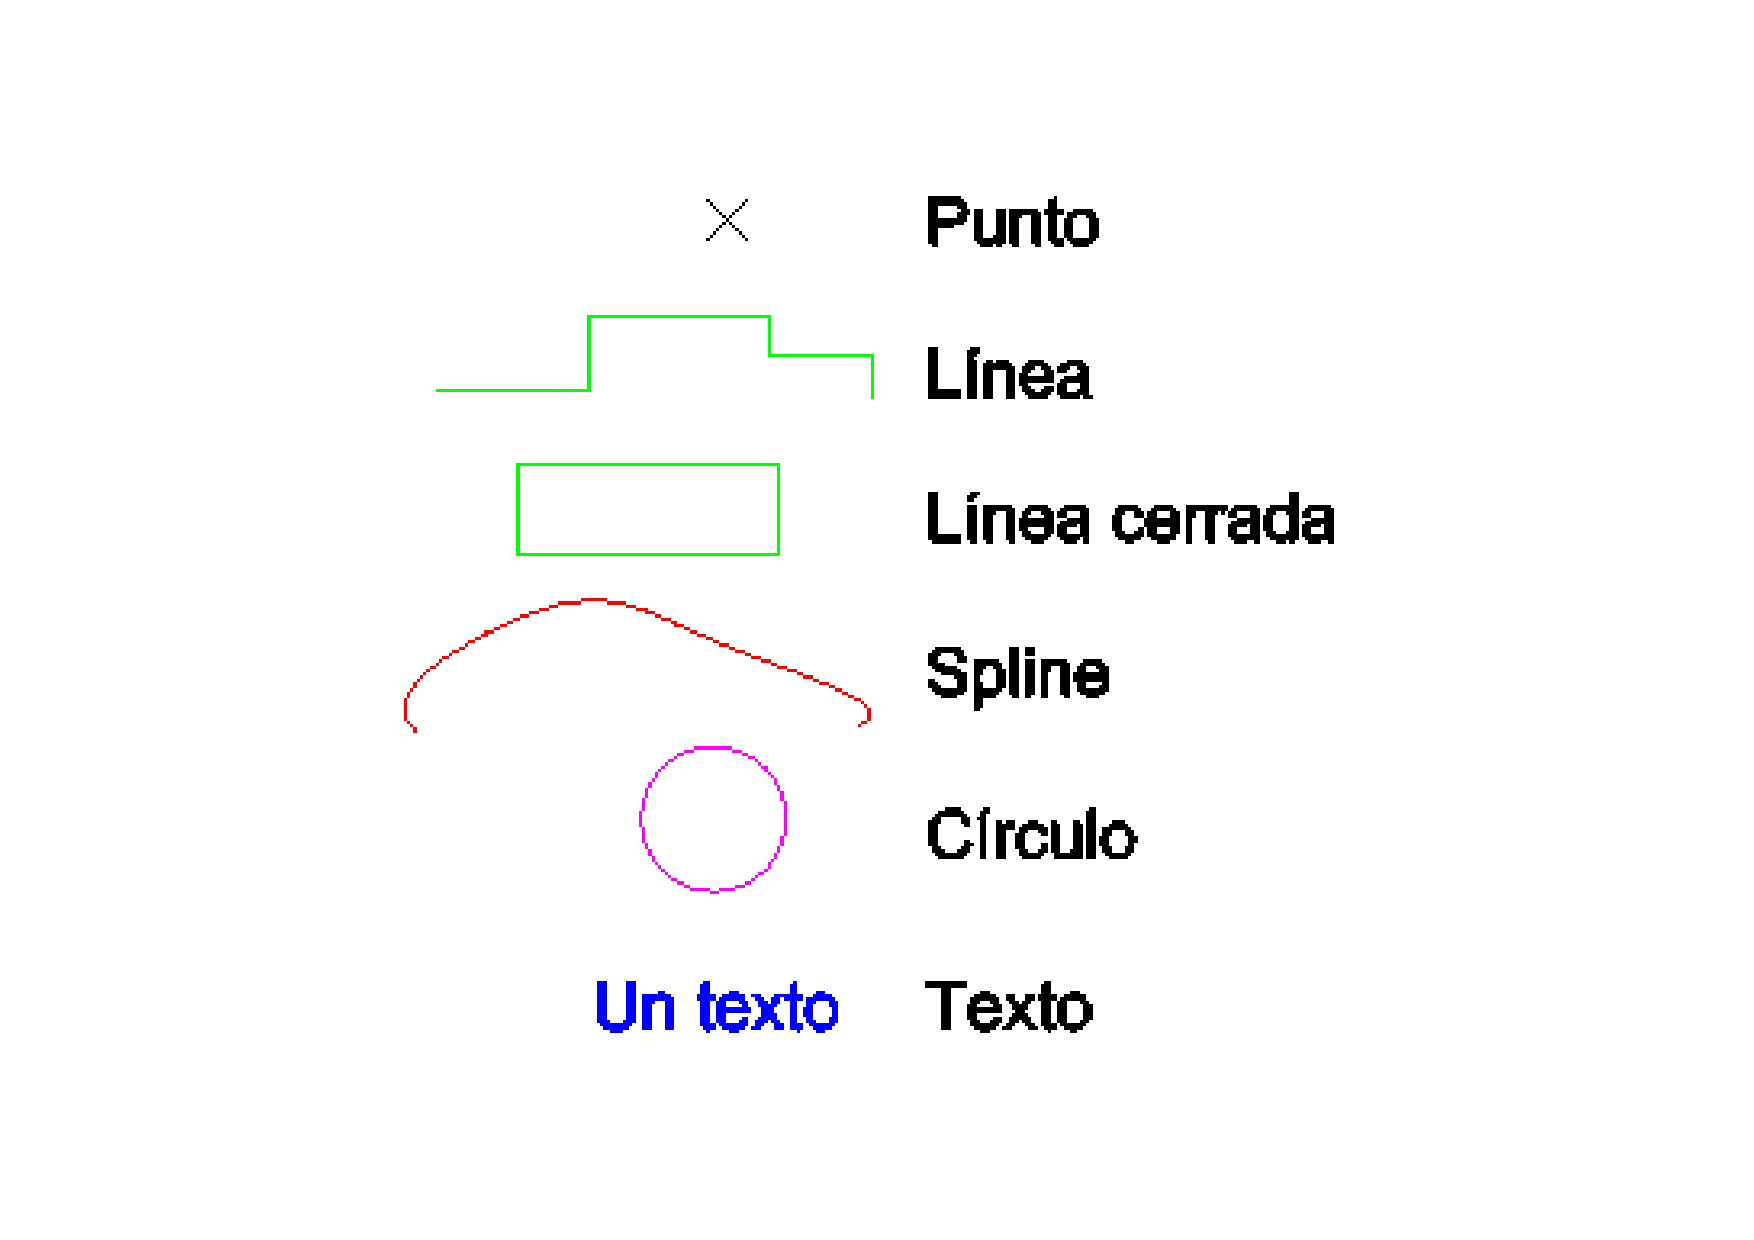
\includegraphics[width=0.5\textwidth]{Tipos}
	\caption{Elementos gráficos.}
	\label{fig:Tipos}
\end{figure}

\newpage

\textbf {Elementos no gráficos}

\begin{itemize}

\item\textbf{Capas:} Sirven para organizar mejor los objetos en nuestro dibujo ayudando a un mejor manejo a la hora de mover, copiar o identificarlos en el plano. Estas son un aspecto fundamental en el desarrollo del dibujo para poder obtener un plano bien organizado y con excelente presentación. En un buen trabajo, es casi imprescindible el uso de capas.

Las capas son una forma de clasificar objetos en CAD, si tienes un plano muy extenso con muchos objetos, la forma más fácil de identificarlos es mediante su capa, cada objeto dibujado en CAD se le asociara una capa y esa capa la puedes crear asignándole un nombre y un color, entre otras cosas. Es la mejor forma de identificar cierto objeto dentro de tu dibujo.
En esta aplicación, las capas tendrán un nombre y un color.

\imagen{capas}{Capas en un programa de CAD}

\item\textbf{Bloques:} Un bloque en CAD es un conjunto de objetos (llamados entidades), agrupados como un todo. Es decir, que podemos dibujar líneas, arcos, círculos, cada uno con propiedades distintas que los demás y luego invocar un comando para <<juntarlos>> a todos bajo un mismo nombre y asignarle un punto de inserción.

En esta aplicación se pretende que el usuario pueda subir un archivo DXF personalizado con sus bloques, y poder asignarlo a diferentes puntos del levantamiento topográfico a través del código de punto


\begin{figure}[!h]
	\centering
	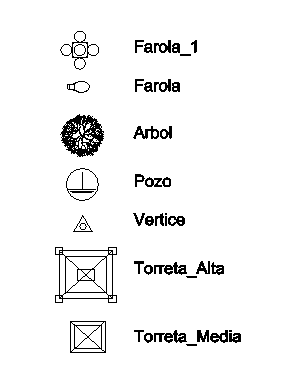
\includegraphics[width=0.4\textwidth]{Simbolos}
	\caption{Símbolos creados como entidades bloques de CAD.}
	\label{fig:Simbolos}
\end{figure}

\end{itemize}

\section{Codificación de los puntos}\label{sec:codificacion}

Como se ha mencionado anteriormente, la codificación de los puntos es la parte clave para el desarrollo de este proyecto, ya que en ella se va a basar la aplicación a la hora de crear los elementos del dibujo.
Debe poder crear líneas y \emph{splines}, interpretando donde empiezan y acaban. Crear círculos, cuadrados y rectángulos, insertar símbolos o bloques en determinados puntos y, por último, asociar cada elemento su capa correspondiente, con su color asignado.

Todo esto, si eres un usuario con conocimientos en manejo de aplicaciones CAD, se haría de forma manual en su mayor parte. Con una buena definición del código de punto, se tratará de automatizar todo este proceso.
Como ya sabemos, el código debe ser lo mas sencillo posible y a la vez aportar la máxima información posible, dejando que el usuario tenga libertad para elegir los códigos, salvo algunas partes, que deben de tener una sintaxis concreta. 

A continuación, veremos algunos ejemplos de codificación para distintos elementos del dibujo:

\begin{itemize}

\item Se quiere dibujar la línea que define el arcén de una carretera, podríamos escribir en el código del punto; ‘ARCEN’, ‘ARC’, ‘A’, o lo que quisiéramos. Como se pretende que el código sea lo más sencillo posible, tomamos como mejor opción ‘A’. Para definir que la línea empieza en un punto concreto, ese texto debe ir seguido obligatoriamente del carácter ‘I’. Un ejemplo de cómo sería una línea de arcén formada por 4 puntos es: (‘A I’, ‘A’, ‘A’, ‘A’).


\begin{figure}[!h]
	\centering
	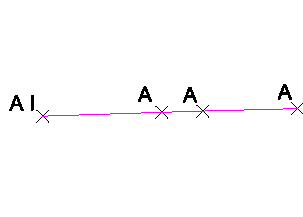
\includegraphics[width=0.6\textwidth]{Polilinea}
	\caption{Representación de una línea.}
	\label{fig:Polilinea}
\end{figure}

\item Siguiendo con el ejemplo anterior, ahora queremos que dibuje una curva tipo \emph{spline}. Para definir que la línea empieza en un punto concreto y que sea \emph{spline}, ese texto debe ir seguido obligatoriamente del carácter ‘IC’ y el resto de los puntos de esa curva, el texto inicial debe ir seguido obligatoriamente del carácter ‘C’. Un ejemplo de cómo sería una línea de arcén tipo \emph{spline} formada por 4 puntos es: (‘A IC’, ‘AC’, ‘AC’, ‘AC’).

\begin{figure}[!h]
	\centering
	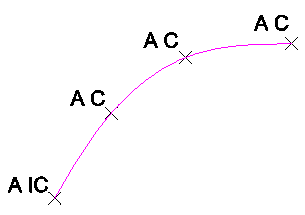
\includegraphics[width=0.6\textwidth]{Splines}
	\caption{Representación de una curva \emph{Spline}.}
	\label{fig:Splines}
\end{figure}

\item Se quiere dibujar un cuadrado, por ejemplo, una tapa de registro perteneciente a la red de saneamiento. El código de punto debe comenzar obligatoriamente por ‘TC’, seguido de la descripción que queramos asignarle, en este caso como es la red de saneamiento usaremos ‘SAN’. Así finalmente, el código para ese punto queda ‘TC SAN’. Como se pretende optimizar también el trabajo de campo, un cuadrado solo se definirá mediante 2 puntos y la aplicación al interpretar el código, deberá siempre dibujar un cuadrado a la derecha de esos dos puntos. La explicación es sencilla, si en un trabajo hay que medir 500 tapas de registro, no es lo mismo medir 1000 puntos que 2000. Con esta codificación nos hemos ahorrado la mitad del tiempo en el trabajo de campo.

\item Lo mismo que en el caso anterior, para dibujar rectángulos. El código de punto debe comenzar obligatoriamente por ‘TR’, seguido de la descripción que queramos asignarle, en este caso como es la red de saneamiento usaremos ‘SAN’. Así finalmente, el código para ese punto queda ‘TR SAN’. Como se pretende optimizar también el trabajo de campo, un rectángulo solo se definirá mediante 3 puntos y la aplicación al interpretar el código, deberá siempre dibujar un rectángulo.

\item Se quiere dibujar un círculo, por ejemplo, una tapa de registro perteneciente a la red eléctrica.  El código de punto debe comenzar obligatoriamente por ‘TX’, seguido de la descripción que queramos asignarle, en este caso como es la red de eléctrica usaremos ‘RE’. En este código necesitaremos también incluir en radio de la circunferencia, por ejemplo 0.5 metros, por lo que al final el código queda ‘TX 0.5 RE’.


\begin{figure}[!h]
	\centering
	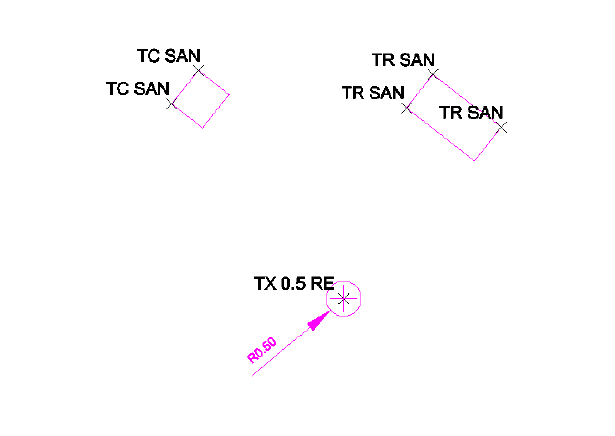
\includegraphics[width=0.8\textwidth]{CRC}
	\caption{Representación de un rectángulo, un cuadrado y un círculo.}
	\label{fig:CRC}
\end{figure}

\item Por último, planteamos una opción más complicada, que suele ser habitual en los trabajos de campo, la representación de elementos que realmente no se han medido en campo, porque pueden no ser accesibles. Queremos representar la línea de la fachada de un edificio, donde existen dos puntos inaccesibles, que no podemos medir topográficamente, pero conocemos su longitud (por ejemplo, hemos extraído estos datos de un plano catastral). Como es un edificio, podríamos representarlo con el texto ‘E’. La siguiente secuencia de 4 puntos con su codificación, construirá la línea final formada por 6 puntos, (‘E I’,’E 1.5 -2’,’E’,’E’). El código el punto 2, ’E 1.5 -2’, indica que cuando la línea llegue a ese punto, debe continuar perpendicular a su derecha durante 1.5 metros, después, 2 metros, también en perpendicular, hacia su izquierda, y por último debe unirse con el siguiente punto que forma la línea. 

\begin{figure}[!h]
	\centering
	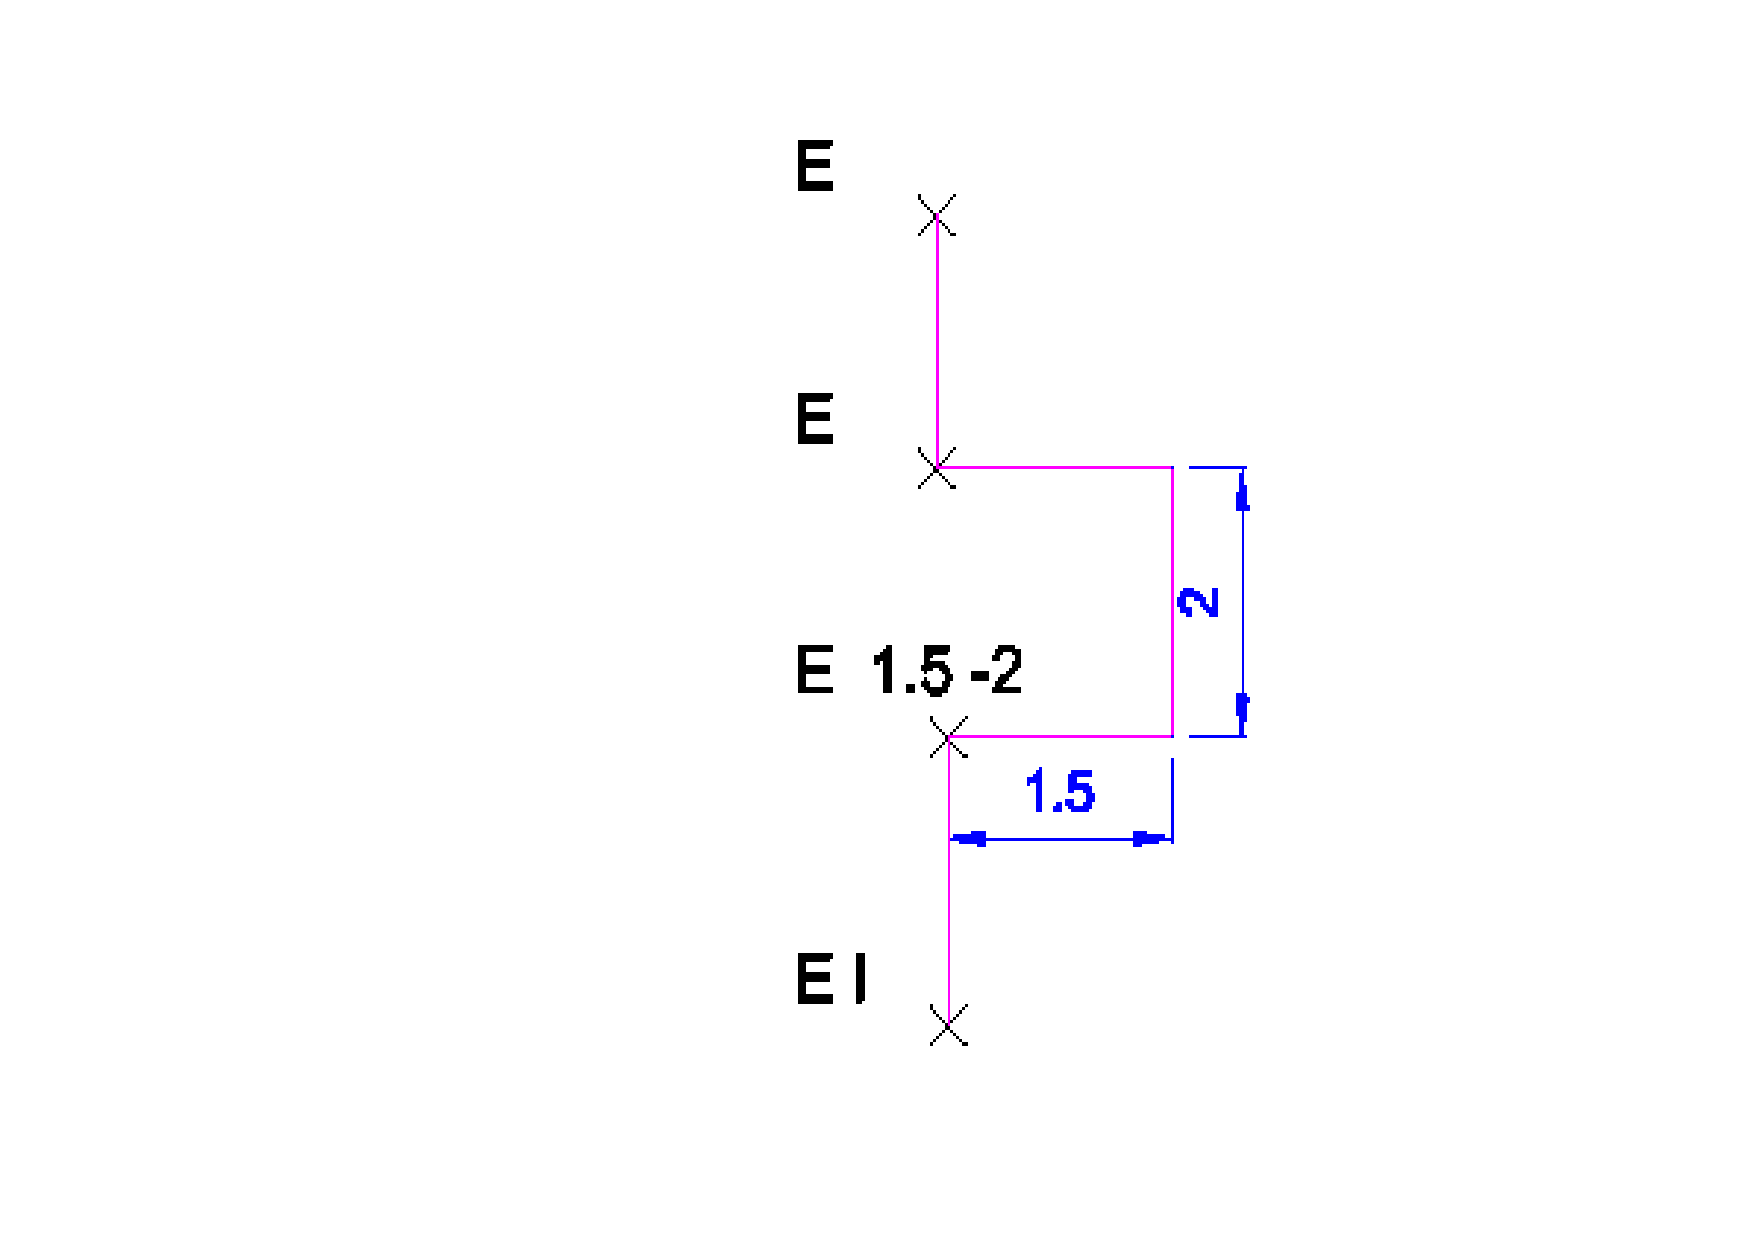
\includegraphics[width=0.6\textwidth]{Inaccesibles}
	\caption{Representación de como se crearía una línea formada por puntos inaccesibles.}
	\label{fig:Inaccesibles}
\end{figure}


\end{itemize}

Otra gran ventaja que aporta esta codificación es que los puntos en campo que forman un elemento no estás obligado a medirlos de forma consecutiva, lo que supone un importantísimo ahorro de tiempo. Vamos a explicar esto con un ejemplo.

Se pretende dibujar el plano de una carretera de 50 km, las líneas que nos interesan son; el eje de la carretera y las líneas de los arcenes. No podemos plantearnos el medir las líneas de forma consecutiva, por ejemplo, medir el arcén derecho, volver por el eje y, por último, el arcén izquierdo. Si hiciéramos esto, recorreríamos 150 km. Esta aplicación es capaz de crear distintas líneas, aunque no estén medidas en campo en un orden consecutivo. Una solución de codificación podría ser la siguiente secuencia de puntos: (‘AD I’,’E I’,’AI I’,’AI’,’E’,’AD’,’E’,’AD’,’AI’,…), donde ‘AD’ es el arcén derecho, ‘E’ el eje, ‘AI’ el arcén izquierdo. Así solo recorreríamos la carretera una sola vez. 

Vemos que este tipo de codificación definida no solo aporta la ventaja de generar automáticamente el plano, si no que, el tiempo ahorrado en el trabajo de campo, es la mayor ventaja. Esta parte del trabajo es la que tiene mayores costes y, por lo tanto, más peso a la hora de decidirse por un proyecto.

\tablaSmall{Caracteres obligatorios y significado.}{l c 
}{codigos}
{ \multicolumn{1}{l}{Caracter} & Significado \\}{ 
'I'	& Punto inicio de línea\\
'IC'& Punto inicio de curva\\
'C' & Punto perteneciente a una curva\\
'TC'& Punto perteneciente a un cuadrado\\
'TR'& Punto perteneciente a un rectángulo\\
'TX'& Punto que define un círculo\\
}
\capitulo{4}{Técnicas y herramientas}
\section{Metodologías}

Como metodología para el desarrollo del proyecto se ha utilizado \textbf {Scrum}.
Scrum es un marco de trabajo, es el método ágil de desarrollo de Software más utilizado del mundo.
Entre sus características principales están:
Utilizar una estrategia de desarrollo incremental, en lugar de la planificación y ejecución completa del producto. 
La calidad del resultado obtenido depende más del conocimiento tácito de las personas que de la calidad de los procesos usados. 
Este método permite el solapamiento entre diferentes fases del proyecto.
Algunos de sus componentes principales son: 
Sprint: Parte básica en este tipo de desarrollos, donde se desarrolla un incremento del producto que pueda ser utilizado.
Pila del producto: donde están los requisitos de usuario, está información no es rígida, puede variar según va evolucionando el producto.
Pila del sprint: lista con las tareas a realizar durante un sprint.
Incremento: Parte del desarrollo obtenida al final de cada sprint.

Durante todo el proyecto se han ido realizando los diferentes sprints, en los cuales se han planificado las tareas siguientes y revisado, si se han ido cumpliendo los objetivos marcados en el sprint anterior.


\section{Patrones de diseño}

Flask utiliza como patrón de diseño, \textbf {MTV}.
El patrón MTV es similar al conocido MVC, pero con algunas diferencias:

En el patrón MVC:
\begin{itemize}
\item\textbf{Modelo:} Es la parte que manipula la información.
\item\textbf{Vista:} Decide como se mostrará la información.
\item\textbf{Controlador:} Comunica el modelo con la vista.
\end{itemize}
Podemos ver a continuación sus equivalencias, para este caso, usando el framework Flask:


\begin{flushleft}
\textbf{\emph{MVC vs	MTV\\}}
Modelo=Modelo\\
Vista=Vista y Template\\
Controlador=Flask\\
\end{flushleft}



Aquí, el framework Flask, es el que toma el papel del controlador.
Resumiendo, en el patrón MTV, tenemos:
\begin{itemize}
\item\textbf{Modelo:} Es la parte que manipula la información, se encuentra en forma de clases de Python.
\item\textbf{Vista:} Decide qué información se muestra y en que template.
\item\textbf{Template:} Coge toda la información, la organiza y ve la manera en que esta se va a mostrar. Básicamente una página HTML con algunas etiquetas extras propias de Flask
\end{itemize}

\imagen{MTV}{Esquema de un patrón MTV}

En la imagen anterior podemos ver como son las relaciones en el patrón MTV:
\begin{enumerate}
\item El Navegador manda una solicitud 
\item La vista interactúa con el modelo para obtener datos. 
\item La vista llama a la plantilla. 
\item La plantilla renderiza la respuesta a la solicitud del navegador 
\end{enumerate}

\section{Control de Versiones}

Existen varias herramientas en el mercado para el control de versiones:
\begin{itemize}
\item Git
\item Subversion
\item SourceSafe
\end{itemize}

Nos hemos decantado por \textbf {Git}, ya que es la que se ha venido usando durante la realización del grado y es una de las mas extendidas en el mercado.

Git es un sistema de control de versiones distribuido, libre y de código abierto. Git se distribuye bajo la licencia de software libre GNU LGPL v2.1. 

\section{Hosting del repositorio}

Al igual que en el apartado anterior, aunque existen diversas posibilidades:
\begin{itemize}
\item GitLab
\item GitHub
\item Bitbucket
\end{itemize}

Como en el apartado anterior, por familiaridad con la plataforma durante el grado y también por ser una de las más usadas, de decidió usar \textbf {GitHub}.

GitHub permite tener cuentas gratuitas y de pago. Además, un tipo de cuenta para estudiantes, como alumno se puede solicitar acogerte al programa «GitHub education for students», que te permite tener repositorios privadas y da acceso a herramientas adicionales.

Además, GitHub ofrece otras funcionalidades y servicios como, por ejemplo; revisión de código, documentación, gestión de tareas, wikis e integraciones con otros servicios como por ejemplo CodeBeat.

\section{Gestión del proyecto}

Dentro de las muchas herramientas existentes como por ejemplo;
\begin{itemize}
\item ZenHub
\item Trello
\item VersionOne
\end{itemize}

Se ha optado por usar  \textbf {ZenHub} ya que se encuentra integrado en el propio GitHub, funciona como una aplicación nativa en su interfaz y podemos controlar nuestros proyectos usando paneles de trabajo bastante intuitivos, así como conectar con varios repositorios en el panel de tareas y ver todos los temas abiertos que requieren de la atención.

Se trata de una plataforma de gestión de proyectos de software y entre las principales características de ZenHub están la de convertir los issues de GitHub en dinámicos tablones Kanban.

\section{Entorno de desarrollo integrado (IDE)}


\subsubsection{Python}

Como en los apartados anteriores se han tenido en cuenta diferentes herramientas para este trabajo:
\begin{itemize}
\item NotePad ++
\item Sublime Text
\item Microsoft Visual Studio Code
\item PyCharm
\end{itemize}

Tanto Microsoft Visual Studio Code como PyCharm son perfectamente válidas y las más completas para realizar este tipo de proyectos, abarcan casi todos los lenguajes de programación, contienen bastantes plugins y facilitan el trabajo a la hora de realizar los test.

Al final nos hemos decantado por \textbf{PyCharm}. Al haberse realizado el proyecto con Python, este entorno ha sido diseñado para este lenguaje, por lo que ofrece algunas ventajas más, respecto a Microsoft Visual Studio Code. PyCharm es soportado por Windows, Mac OS y Linux, y su versión gratuita es bastante completa. Existen también licencias individuales para estudiantes.



\subsubsection{\LaTeX}
La documentación del proyecto ha desarrollado en \LaTeX. Para este propósito se han tenido en cuenta las siguientes herramientas:
\begin{itemize}
\item MikTex, para SO Windows
\item texlive, para SO Linux
\item MacTex, para SO Mac
\item Compatible con las 3 plataformas, Texmaker
\item Editor en línea, overleaf
\end{itemize}

Se ha optado por \textbf{Texmaker}, como recomendación del tutor del proyecto.
Integra la mayoría de herramientas necesarias para la escritura de documentos en \LaTeX, es gratuito y tiene licencia GNU GPL v2.

\section{Servicios de integración continua}


\subsubsection{Calidad del código}
Las diferentes herramientas consideradas para este propósito han sido: 
\begin{itemize}
\item SonarQube
\item CodeBeat
\end{itemize}

Se ha optado por \textbf{CodeBeat}, ya que se integra perfectamente con GitHub. Es una herramienta gratuita, que soporta gran cantidad de lenguajes y permite personalizar totalmente, las métricas que usa para el análisis de la calidad del código.

\section{Herramienta de análisis sintáctico}

Como herramienta de análisis sintáctico, para poder dar validez a los archivos de entrada, se pensó en estas 3 posibilidades:
\begin{itemize}
\item Ply
\item Antlr
\item Flex Bison
\end{itemize}

La opción elegida ha sido \textbf{Ply}, ya que está implementada completamente en Python y encaja perfectamente con la filosofía de realizar la mayor parte del proyecto con este lenguaje.

Aunque Ply también es una librería y debería estar en el apartado de librerías, le hemos querido dar un apartado especial como herramienta de análisis sintáctico.

Ply es una biblioteca de Python. Es una implementación de lex y yacc de herramientas de análisis para Python, que proporciona la mayor parte de las características estándar de lex / yacc, incluyendo; el apoyo a las producciones vacías, las reglas de prioridad, la recuperación de errores y soporte para gramáticas ambiguas. Es muy sencillo de usar y también muy efectivo a la hora de realizar la comprobación de los errores. Ply utiliza el análisis LR, el cual puede incorporar grandes gramáticas fácilmente.

Ply, básicamente está compuesto de 2 módulos:
\begin{itemize}
\item ply.lex – Donde se trata la parte del análisis léxico
\item ply.yacc -  Este módulo es para crear un parser.
\end{itemize}

\section{Librerías}

A continuación, vemos el resto de las librerías necesarias en el desarrollo de este proyecto:


\subsubsection{ezdxf}

ezdxf es la librería más importante del proyecto. En un principio, se tuvieron en cuenta otras opciones como:
\begin{itemize}
\item dxfgrabber
\item SDXF
\item dxfwrite
\end{itemize}

resultando la opción más interesante ezdxf, ya que era la única que cubría todas las necesidades que aquí se planteaban.

\textbf{ezdxf} es una interfaz de Python para el formato DXF, desarrollado por Autodesk, y que permite a los desarrolladores leer y modificar dibujos DXF existentes o crear nuevos dibujos DXF.

Con sus métodos y atributos nos permite crear, modificar, eliminar o consultar las propiedades de todos los elementos que puede contener un archivo de CAD.
ezdxf es independiente del sistema operativo y se ejecuta en todas las plataformas que proporcionan un intérprete de Python adecuado (> = 3.6). Esta bajo la licencia MIT-License.

Una parte a destacar, es que nos permite generar el DXF en distintas versiones de un archivo CAD, lo cual es muy interesante. 

\imagen{Cad_versions}{Versiones de CAD}

\subsubsection{SQLAlchemy}

Se ha elegido la librería de Python \textbf{SQLAlchemy} por que es el ORM que mejor se adapta para trabajar con Flask y PostgreSQL

\subsubsection{Flask-Login}

Se ha elegido la librería de Python \textbf{Flask-Login} para poder realizar la gestión de sesiones de usuarios en la aplicación.


\subsubsection{Bootstrap}

\textbf{Bootstrap} es un framework para desarrollo front-end. Permite crear de forma sencilla webs de diseño adaptable, es decir, que se ajusten a cualquier dispositivo y tamaño de pantalla y siempre se vean igual de bien.
Es una herramienta Open Source


\subsubsection{Colorpicker Bootstrap}

\textbf{Colorpicker Bootstrap},  es un plugin de selector de color modular para Bootstrap 4. Esta bajo la licencia MIT-License.


\subsubsection{TinyColor}

Es un micro framework que permite la manipulación y conversión de color en JavaScript. Permite muchas formas de entrada, mientras que proporciona conversiones de color y otras funciones de utilidad de color. No tiene dependencias. Esta bajo la licencia MIT-License


\subsubsection{bs-custom-file-input}

\textbf{bs-custom-file-input} ,es un plugin para Bootstrap 4. Ayuda a crear una entrada de selección de archivos personalizada con el botón del navegador para cargar archivos. También es compatible con múltiples selecciones de archivos y arrastrar y soltar.
No tiene dependencias. Esta bajo la licencia MIT-License

\section{Desarrollo Web}

Para el desarrollo web se ha optado por utilizar \textbf{Flask}, siguiendo, como se ha comentado anteriormente con la idea de englobar lo máximo posible en Python.
Flask es un “micro” Framework escrito en Python y concebido para facilitar el desarrollo de aplicaciones Web bajo el patrón MTV.

Entre algunas de sus ventajas, están:
\begin{itemize}
\item Desarrollo de aplicaciones web de una forma ágil y rápida, tiene una buena curva de aprendizaje
\item No se necesita una infraestructura con un servidor web.
\item Compatible con wsgi.
\item Soporta de manera nativa el uso de cookies seguras.
\item Se pueden usar sesiones.
\item Flask es Open Source y tiene una licencia BSD.
\item Extensa documentación.
\end{itemize}

\section{Despliegue de la aplicación}

Para el despliegue de la aplicación se ha optado por utilizar \textbf{Docker}. Principalmente, porque es una herramienta de mucha actualidad y con un gran potencial, tanto en el desarrollo, como en el despliegue de aplicaciones.

La idea básica de su funcionamiento es la creación de una serie de contenedores muy ligeros y portables, así las aplicaciones, podrán ejecutarse en cualquier equipo, solamente con tener Docker instalado, con independencia del sistema operativo.

Entre algunas de sus ventajas, están:

\begin{itemize}
\item Es muy sencillo de usar.
\item Ahorra tiempo, no necesitamos instalar diferentes softwares.
\item Son muy ligeros, a diferencia de las máquinas virtuales ya que no necesitan un sistema operativo completo, cogen lo que necesitan de cada máquina anfitriona.
\item Portabilidad.
\item Los repositorios Docker, nos permite acceder a gran cantidad de imágenes y así poder de ejecutar prácticamente todas las aplicaciones.
\item Es un entorno seguro y no ofrece variaciones, da igual cual sea el equipo ni el ambiente. Facilita las pruebas, el desarrollo y las visualizaciones por parte del cliente.
\item Es Open Source.
\item Extensa documentación.
\end{itemize}

\capitulo{5}{Aspectos relevantes del desarrollo del proyecto}

Este apartado pretende recoger los aspectos más importantes del desarrollo del proyecto. Se tratará de exponer el camino que se ha tomado con sus correspondientes implicaciones, así como describir los diferentes problemas a
los que ha habido que enfrentarse y las soluciones con las que se ha tratado de resolverlos.

\section{Inicio del proyecto}

Me considero una persona con muchas inquietudes y siempre pensando en mejorar tareas que suelo realizar con mucha frecuencia. He desarrollado mi carrera profesional en el campo de la Topografía y la Geodesia, y actualmente está mas enfocado a temas relacionados con la Cartografía.

Trabajando en varios proyectos, he podido observar la cantidad de tiempo y recursos que se empleaban, en realizar levantamientos topográficos y posteriormente gestionar todos esos datos para producir un plano. De ahí surge la idea de como mejorar el trabajo de campo mediante un tipo de codificación,  y que esta a su vez sirviera para automatizar al máximo el proceso de delineación, a la hora de  crear el plano.

El profundizar en los conocimientos adquiridos cursando el Grado en Ingeniería Informática y a la vez poder facilitar el trabajo en este tipo de proyectos, me ha animado a hacer viable este proyecto. A la hora de decidirme, también me ha parecido importante, la idea de que la aplicación desarrollada es de gran utilidad, y seguro que va a ser bien recibida por la comunidad de topógrafos.

La idea fue aceptada por los tutores, y comenzamos con el proyecto.

\begin{figure}[!h]
	\centering
	
\includegraphics[width=0.4\textwidth]{SPC}
	\caption{Logo de \emph{SurveyingPointCode}.}
	\label{fig:SPC}
\end{figure}


\section{Gestión del proyecto}

En la primera reunión con los tutores, se estableció cual iba a ser la metodología a seguir en la realización de este proyecto. Se iba a emplear la metodología ágil \emph{Scrum}.

Se realizarían una serie de \emph{sprints} llevados a cabo con una periodicidad media semanal, donde se entregaría una parte del producto operativo, el incremento. Al finalizar cada \emph{sprint} se realizarían reuniones para planificar las tareas a realizar en el el \emph{sprint} siguiente, en forma de pila del \emph{sprint}, y revisar si se habían alcanzado los objetivos marcados en el \emph{sprint} anterior.

En \emph{GitHub}, con la herramienta \emph{ZenHub}, se visualizarían el estado y prioridad de las tareas del \emph{sprint}. Los avances y cambios en el desarrollo del proyecto, se almacenaría en \emph{GitHub}, que nos permitiría seguir al detalle  todo el histórico del proyecto.

Las reuniones de los \emph{sprints} resultaron muy interesantes. En ellas hubo modificaciones sobre la idea inicial de la que se partía, en algunos casos desechado alguna funcionalidad, como la de incorporar un visor para poder visualizar el plano en el navegador (véase la explicación en el \emph{sprint} 6, en el anexo), pero en la mayoría de los casos, aportando nuevas funcionalidades que hacían  crecer el valor de la aplicación, y sobre todo me aportaron una visión más realista a la hora de abordar unos determinados objetivos o ideas, preguntándome, si el tiempo o recursos invertidos merecían la pena o aportaban algún valor a la aplicación.

\section{Formación}

La realización del proyecto requería una serie de conocimientos técnicos, en general, en el desarrollo de aplicaciones web,y en particular en  tecnologías como;
Flask, HTML5, CSS3, JavasScript, Docker y bilbliotecas como \texttt{Ply}, \texttt{ezdxf}, \texttt{Boostrap}, \texttt{TinyColor},...

Los mayores esfuerzos se pusieron en comprender el funcionamiento de Flask, \texttt{Ply}, \texttt{ezdxf} y Docker, ya que el óptimo funcionamiento de la aplicación  en estos puntos, era fundamental para logar conseguir los objetivos finales. 

Como la aplicación se ha desarrollado en Python, era importante conocer las guías de estilo y la convenciones de este lenguaje, \textbf{PEP 8} y \textbf{PEP 257} entre otras. Para ello se consultaron las siguientes fuentes:

\begin{itemize}
\item PEP 8 -- Style Guide for Python Code \cite{PEP8}
\item PEP 257 -- Docstring Conventions \cite{PEP257}
\end{itemize}


Para la formación en \textbf{Flask} se consultaron las siguientes fuentes:

\begin{itemize}
\item Building Web Applications  with Flask \cite{Flask1}
\item Instant Flask Web Development \cite{Flask2}
\end{itemize}

Para la formación en \textbf{Ply} se consultaron las siguientes fuentes:

\begin{itemize}
\item Documentation for PLY  \cite{HomePly}
\item Prototyping Interpreters using Python Lex-Yacc \cite{Ply2}
\item Parses chemical equations using the PLY parser generator \cite{Ply3}
\end{itemize}

Para la formación en \textbf{ezdxf} y las otras posibles alternativas,se consultaron las siguientes fuentes:

\begin{itemize}
\item Documentation for ezdxf \cite{ezdxf}
\item Documentation for dxfgrabber \cite{dxfgrabber}
\item Documentation for dxfwrite \cite{dxfwrite}
\item Documentation for SDXF \cite{sdxf}
\end{itemize}

Para la formación en \textbf{SQLAlquemy}  y \textbf{Flask-Login}, se consultaron las siguientes fuentes:

\begin{itemize}
\item Documentation for SQLAlquemy \cite{SQLAlquemy}
\item Documentation for Flask-Login \cite{Flasklogin}
\end{itemize}

Para la formación en \textbf{HTML5} se consultaron las siguientes fuentes:

\begin{itemize}
\item HTML5 Tutorial \cite{html5}
\end{itemize}

Para la formación en \textbf{CSS3} se consultaron las siguientes fuentes:

\begin{itemize}
\item CSS Tutorial \cite{css3}
\item Lenguaje CSS \cite{css3_1}
\end{itemize}

Para la formación en \textbf{JavaScript} se consultaron las siguientes fuentes:

\begin{itemize}
\item Eloquent JavaScript: A Modern Introduction to Programming \cite{JavaScript}
\item Javascript a fondo \cite{JavaScript_1}
\end{itemize}

Para la formación en \textbf{Bootstrap} y bilbliotecas relacionadas, se consultaron las siguientes fuentes:

\begin{itemize}
\item Bootstrap \cite{Bootstrap}
\item TinyColor JavaScript color tooling \cite{TinyColor}
\item Bootstrap Colorpicker \cite{Colorpicker}
\item jquery.cookie \cite{j-cookie}
\end{itemize}


Para la formación en \textbf{Docker} se consultaron las siguientes fuentes:

\begin{itemize}
\item Curso Docker \cite{Docker}
\item Docker for beginners \cite{Docker_1}
\item Introduction to Docker \cite{Docker_2}
\item Docker-postgis \cite{Docker_3}
\item Overview of Docker Compose \cite{Docker_4}
\end{itemize}

\section{Desarrollo de la aplicación}

Los primeros pasos en el desarrollo de la aplicación consistieron en desarrollar un pequeño prototipo funcional, que fuera incrementando su funcionalidad progresivamente.

El primer prototipo, tenía que conseguir leer un archivo de campo y darlo por válido o como erróneo. Una vez que se tuvo clara como iba a ser la codificación de cada punto, (según hemos visto en la Sección~\ref{sec:codificacion} en la página~\pageref{sec:codificacion}), el siguiente paso era definir una gramática para ese tipo de archivo, para poder validarla. Entre los formatos de archivo más comunes que podemos obtener de los equipos topográficos, se decidió que los archivos deberían ser de tipo <<csv>> o <<txt>>, separando sus campos por comas. Los campos son; número de punto, coordenada $x$, coordenada $y$, coordenada $z$ y código del punto. 

A continuación, vemos un ejemplo, con todas las posibilidades de codificación que aceptará la aplicación: 
\begin{verbatim}


1,355776.180,4611015.011,691.055,E I
2,355773.203,4611028.546,691.055,E
3,355781.359,4611129.076,691.055,TR REG
4,355786.052,4611135.542,691.055,TC TEL
5,355783.215,4611143.179,691.055,TX 2 SAN
6,355754.037,4611145.893,691.055,A IC
7,355755.345,4611150.953,691.055,A C
8,355857.822,4611095.993,691.055,E -14.1 20.5 -25.75
\end{verbatim}



Se estudió detenidamente esta sintaxis y la formalización de la gramática quedó de la siguiente forma:

\begin{verbatim}
entrada: líneas

líneas: línea | líneas '\n' línea

línea: núm_punto coordenadas código

núm_punto: INT

coordenadas: FLOAT, FLOAT, FLOAT

INT: [0-9]+

FLOAT: -?( [0-9]*.[0-9]+)

ID: [a-zA-Z]+

código: código_capa CÓDIGO_GEOMÉTRICO
      | CÓDIGO_ELEMENTO_SINGULAR código_valor_texto
      | código_capa código_no_accesible
      | código_elemento_singular
      | código_capa      
      
código_capa: ID

CÓDIGO_GEOMÉTRICO: "I" | "IC" | "C"

CÓDIGO_ELEMENTO_SINGULAR: "TC" | "TR" | "TX"

código_valor_texto: FLOAT ID
                  | INT ID
                  | FLOAT
                  | INT
                  | ID       
                                 
código_no_accesible: (FLOAT | INT)+
\end{verbatim}

El prototipo utilizando la biblioteca \texttt{Ply} y con esta gramática,  consiguió validar un archivo correcto.

Otro punto clave en el desarrollo del algoritmo fue descifrar los códigos que contenía el archivo de entrada. Como se ha comentado anteriormente, este código puede tener distintos significados dependiendo de su estructura, por ejemplo:

\begin{itemize}
\item AR, puede ser un punto que se guarde en una futura capa llamada Árboles.
\item TX 2 SAN, puede ser un punto que es el centro de un circulo de radio 2 y que se guarde en una futura capa llamada Saneamiento.
\item M I, puede ser un punto donde comienza una línea que define un muro y que se guarde en una futura capa llamada Muros.
\item …
\end{itemize}

El algoritmo debía extraer del archivo todos los elementos, identificarlos y guardarlos en alguna estructura de datos, clasificados por:

\begin{itemize}
\item Capas
\item Puntos
\item Líneas
\item Curvas
\item Cuadrados
\item Rectángulos 
\item Círculos
\end{itemize}

Añadiendo complejidad al archivo de entrada, se comprobó que el algoritmo resolvía de forma satisfactoria este paso.

Por último, para poder tener un prototipo básico que cumpliera los objetivos, debíamos comprobar que el prototipo era capaz de crear un archivo \textbf{DXF}, con los elementos del archivo de entrada. Incorporando la biblioteca \texttt{ezdxf}, y haciendo uso de sus métodos y atributos, se testó que dibujara en un primer momento solo líneas y curvas, siendo capaz de generarlas en el orden correcto.

Con estos datos de entrada:

\begin{verbatim}

1,355776.180,4611015.011,691.055,E I
2,355773.203,4611028.546,691.055,E
3,355761.305,4611083.365,691.055,E
4,355767.050,4611086.462,691.055,A I
5,355774.447,4611083.001,691.055,M I
6,355769.692,4611104.977,691.055,M
7,355763.294,4611103.572,691.055,A
8,355756.420,4611105.247,691.055,E
9,355781.359,4611129.076,691.055,TR RE
10,355782.355,4611131.314,691.055,TR RE
11,355788.919,4611128.392,691.055,TR RE
12,355766.146,4611121.294,691.055,M
13,355759.713,4611119.882,691.055,A
14,355750.443,4611133.259,691.055,E
15,355786.052,4611135.542,691.055,TC TEL
16,355786.849,4611136.145,691.055,TC TEL
17,355764.814,4611134.156,691.055,ARB
18,355783.215,4611143.179,691.055,TX 0.5 SAN
19,355761.943,4611140.629,691.055,M
20,355755.486,4611139.240,691.055,A
21,355754.037,4611145.893,691.055,A IC
22,355745.977,4611153.511,691.055,E
23,355755.345,4611150.953,691.055,A C
24,355758.897,4611153.511,691.055,A C
\end{verbatim}

El resultado fue:

\imagen{proto_1}{Dibujo obtenido con el prototipo inicial}


Es resultado fue el esperado, por lo que se concluyó esta primera etapa del desarrollo con un pequeño prototipo que cumplía las funcionalidades previstas inicialmente:

\begin{itemize}
\item Leer y validar un archivo con una gramática determinada.
\item Interpretar y organizar todos los elementos del archivo, a partir de su codificación.
\item Crear un archivo DXF con estos elementos.
\end{itemize}

A partir de aquí, como ya se había decidido que iba a ser una aplicación Web, el próximo objetivo era desarrollar la aplicación Web con \textbf{Flask}. El proceso iba a ser el mismo que con el prototipo anterior, desarrollar un prototipo de aplicación Web que fuera incrementando sus funcionalidades.

A continuación, se enumeran brevemente y ordenadas temporalmente, las funcionalidades más importantes que se han ido añadiendo al prototipo Web:
\begin{itemize}
\item Subir un archivo al servidor.
\item Procesar y descargar un archivo al equipo del usuario.
\item Conexión con una BBDD. (en este punto se comenzó a trabajar con Docker, la BBDD iba dentro de un contenedor).
\item \emph{Login}, \emph{Logout} y Registro. Para implementar esta parte se trabajó con la biblioteca \texttt{Flask-Login}.
\item Sesiones de usuarios. 
\end{itemize}

Estas funcionalidades cubrían las expectativas de que la aplicación fuera una aplicación Web, el prototipo Web ya se había conseguido.

A partir de aquí, se han ido desarrollando todas las funcionalidades de la aplicación tanto en \emph{Frontend} como en  \emph{Backend}.

\section{Problemas, incidencias y soluciones}

A continuación, se exponen algunos  problemas surgidos, incidencias y como se abordaron.


\subsubsection{Conflicto entre \emph{parsers}}

Tras obtener el prototipo inicial, con la funcionalidad que se tenía en mente en un principio,  surgió la idea que el usuario pudiera subir un archivo con una configuración personalizada para hacer la conversión de archivo de campo a archivo DXF. 

Como podemos ver en la Tabla~\ref{tabla:config}, relacionamos códigos de punto, con capas de CAD, colores y símbolos. Cuando exista un trabajo con múltiples códigos, capas y colores, se quiere dar al usuario la posibilidad de no tener que configurar cada vez esta conversión en la interfaz, sino que a través de un archivo personalizado, con sus códigos, capas, colores y símbolos, esta parte sea también automática.

\tablaSmall{Esquema archivo de configuración}{l c c c
}{config}
{ \multicolumn{1}{l}{Código de punto} & Capa de CAD & Color & Símbolo \\}{ 
E & Edificación & Rojo\\
AR & Vegetación & Verde & Árbol\\
SAN & Saneamiento & Amarillo \\
P & Saneamiento & Amarillo & Pozo \\
}

Para ello se formalizó otra gramática para validar este tipo de archivos y detectar sus errores. La gramática elegida fue la siguiente:


\begin{verbatim}

entrada: líneas

líneas: línea | líneas '\n' línea

línea: TEXT COMA TEXT COMA color COMA TEXT
     | TEXT COMA TEXT COMA color
     
color: LPAREN INT COMA INT COMA INT RPAREN

TEXT: [a-zA-Z0-9_]+

INT: [0-9]+

LPAREN = '\('

RPAREN = '\)'

\end{verbatim}

Los \emph{parsers} estaban definidos en diferentes módulos, el \emph{parser} para el archivo del campo estaba en módulo \ruta{conversor.py} y el del archivo de configuración en el módulo \ruta{upload\_optional\_files.py}. Cuando se ejecutan, se crean los archivos \ruta{parser.out} y \ruta{parsetab.py}. Probando a cargar los dos archivos a la vez, se pudo comprobar que se parseaba un archivo con el \emph{parser} que no le correspondía. Esto no sucedía siempre, si no que pasaba  de una forma aleatoria, como si en algún momento se cruzara la información entre \emph{parsers}.

Se solucionó esta parte añadiendo un parámetro personalizado para cada tipo de \emph{parser}. En un principio estaba definido de esta forma para ambos casos:
\

\begin{lstlisting}
lex.lex() # lexer part
...
punto = parser.parse(line) # parser part
\end{lstlisting}

Definiendo parámetros independientes en cada caso, quedó de la siguiente forma.

Para el archivo de campo:

\begin{lstlisting}
lexer_topographycal=lex.lex() # lexer part
...
# añadiendo el nuevo parámetro
punto = parser.parse(line,lexer=lexer_topographycal)
\end{lstlisting}
\newpage
Para el archivo de configuración:

\begin{lstlisting}
lexer_config = lex.lex() # lexer part
...
# añadiendo el nuevo parámetro
c_line = parser.parse(line, lexer=lexer_config)
\end{lstlisting}
Para dar con esta solución, se consultó la documentación de \texttt{Ply}, concretamente el apartado \textbf{Multiple Parsers and Lexers} \cite{Parser}.


\subsubsection{Codificación \texttt{UTF-8}}

Hasta ahora la aplicación funcionaba correctamente a la hora de subir los archivos y validarlos. Se decidió modificar la gramática del archivo de configuración, para que aceptará la letra <<ñ>> y todos los tipos de tildes, ya que se suelen utilizar al poner los nombres de las capas de CAD. 

Simplemente se sustituyó:

\begin{verbatim}
TEXT: [a-zA-Z0-9_]+
\end{verbatim}

por: 

\begin{verbatim}
TEXT: [a-zA-ZÀ-ÿ0-9ñÑ_]+
\end{verbatim}


Con esto debería funcionar perfectamente, pero no fue así, el archivo que contenía el carácter <<ñ>>, daba errores. Se estaba probando la aplicación simultáneamente en 2 sistemas operativos Windows y Linux, y para mayor sorpresa en Linux funcionaba y en Windows no.

Al final, se dedujo que se podía tratar de un problema de codificación del archivo, e investigando en esa línea decidimos probar dos configuraciones, \texttt{UTF-8} y \texttt{Latin-1}, en los 2 sistemas , y en cada uno sucedía lo contrario, como se puede ver en la Tabla Tabla~\ref{tabla:WL}


\tablaSmall{Test Windows vs Linux para \texttt{UTF-8} y \texttt{Latin-1}}{l c c c
}{WL}
{ \multicolumn{1}{l}{Sistema Operativo} & UTF-8 & Latin-1 \\}{ 
Windows & Fallo & Correcto\\
Linux & Correcto & Fallo\\
}
 
La solución encontrada fue añadir en la función que abre el archivo, el parámetro \emph{encoding} indicando el tipo de codificación específicamente , en este caso \texttt{UTF-8}. 

En el código se sustituyó:
\begin{lstlisting}
  with open(input_file) as f:
\end{lstlisting}

por:
\begin{lstlisting}
  with open(input_file, encoding='utf-8') as f:
\end{lstlisting}

Se comprobó en ambos sistemas operativos, y el resultado fue correcto, así que se dio esta solución como válida.


\subsubsection{Paleta de colores en CAD}

Una funcionalidad importante de la aplicación es poder asignar un color a una capa de CAD, así todos los elementos pertenecientes a esa capa se dibujarán en ese color. 

La función para crear una nueva capa de la biblioteca \texttt{ezdxf},

\begin{lstlisting}
  dwg.layers.new(nombre_capa, dxfattribs={'color': 1})
  # atributo color, en este ejemplo igual a 1
\end{lstlisting}

\noindent solo permite colores entre 0 y 255, por lo que en un principio, se pensó en usar esta paleta de colores o si la entrada se producía en formato RGB, tanto en el archivo de configuración o a través de la interfaz, se transformaría de RGB a 256 colores, mediante la siguiente trasformación:

\begin{lstlisting}
def rgb(r,g,b):
    grayP=True
    gray=False
    sep=45.5

    while(grayP):
        if (r<sep)or g<sep or b<sep:
            gray=r<sep and g<sep and b<sep
            grayP=False
        sep+=42.5

    if (gray):
        return round(232+(r+g+b)/33)
    else:
        return 16+(6*r/256)*36+(6*g/256)*6+(6*b/256
\end{lstlisting}

El algoritmo anterior se consultó en:

\url{https://github.com/janlelis/paint} 

Con esto se había solucionado el problema, ya teníamos cada capa con su correspondiente color.

Al cabo de bastantes pruebas, apareció un detalle que en un principio me había pasado inadvertido, los colores que seleccionaba el usuario para crear el archivo DXF en la aplicación , no se correspondían con los que realmente se visualizaban en el dibujo, una vez abierto con un programa de CAD.

Investigando, se averiguó que los programas de CAD tienen su propia paleta de colores, que fue creada por AutoCAD, donde a cada color se le asigna un número entero entre 0 y 255. En el siguiente enlace se puede consultar:


\url{http://gohtx.com/acadcolors.php}

Esta parte se solucionó incluyendo en la aplicación, una lista con estos colores, donde se comparaba el RGB definido por el usuario con el de la lista, y si existía, devolvía el número entero correspondiente a la paleta de CAD.

Cuando los colores estaban definidos en el archivo de configuración, no había problema, era una conversión directa usando la lista anterior, pero si el usuario deseaba asignar o modificar el color a través de la interfaz, el color que él había seleccionado debería ser igual al que apareciera en el dibujo. Para ello se utilizó la biblioteca de JavaScript, \texttt{TinyColor}, que nos permite personalizar la paleta de colores con cualquier lista que le proporcionemos.

\imagen{colores_cad}{Ejemplo diez primeros colores en la paleta de colores CAD}

\imagen{colores_app}{Paleta de colores de \emph{SurveyingPointCode}}

En las figuras~\ref{fig:colores_cad} y ~\ref{fig:colores_app}, se puede observar que la disposición de colores está ordenada de la misma forma, coincidiendo su posición con el número entero correspondiente al color de la paleta de CAD.

\subsubsection{Versiones iniciales de CAD}

En un principio de planteó que la aplicación debería poder generar versiones de archivos DXF compatibles con todas las versiones de CAD existentes en el mercado.

En los prototipos iniciales, con los ejemplos de archivos de campo que veníamos trabajando, se comprobó que se generaban archivos DXF válidos para todas las versiones de CAD. Hasta ahora se habían utilizado elementos de CAD, de tipo:

\begin{itemize}
\item \texttt{POINT}
\item \texttt{LWPOLYLINE}
\item \texttt{CIRCLE}
\item \texttt{SPLINE}
\item \texttt{TEXT}
\end{itemize}

Que permitían esta compatibilidad, con las versiones más antiguas.   

La aplicación en un principio estaba pensada para que el usuario pudiera asociar   a determinados códigos de puntos, un símbolo. Por ejemplo, en un punto que tuviera el código AR, debía dibujar un árbol.(Véase un ejemplo de distintos símbolos en la Figura~\ref{fig:Simbolos}).

Se añadió esta nueva funcionalidad, que debía realizar los siguientes pasos:

\begin{itemize}
\item Subir un archivo DXF con bloques.
\item Extraer los bloques que contiene ese archivo.
\item Incorporar esos bloques a nuestro dibujo.
\item Asignar esos bloques a determinados puntos, para que sean dibujados como símbolos.
\end{itemize}

Y el nuevo tipo de elemento añadido \texttt{BLOCK}, hizo que versiones mas antiguas de CAD, no soportaran este formato.

Valorando este problema, se determinó que era mejor desechar el poder trabajar con versiones más antiguas de CAD, en favor, de que el usuario pudiera asignar símbolos al dibujo. Sin esta posibilidad, la aplicación perdería mucho valor.


\begin{figure}[!h]
	\centering
	\includegraphics[width=0.6\textwidth]{cad_versions_ok}
	\caption{Versiones de CAD aceptadas por \emph{SurveyingPointCode}.}
	\label{fig:cad_versions_ok}
\end{figure}


En la Figura~\ref{fig:cad_versions_ok}, podemos ver las versiones de archivos DXF
compatibles en \emph{SurveyingPointCode}

\subsubsection{Despliegue de la aplicación --- Docker Compose.}

Como idea inicial, se planteó el uso de Docker para llevar a cabo el despliegue de la aplicación. Una vez que tengamos bien configurados los contenedores, es sencillo de desplegar en cualquier equipo.

Primero, se configuró el contenedor  de la base de datos, \emph{PostGIS}, junto con \emph{PgAdmin4}, para gestionar la base de datos. Dos contenedores conectados entre sí.

Mas adelante, se pensó crear un contenedor que contuviera la aplicación, configurar un contenedor con \emph{Flask}. Ya teníamos tres contenedores independientes conectados entre sí, y con la aplicación funcionando perfectamente.

Para desplegar la aplicación, había que descargar la imagen de cada contenedor, crear y arrancar cada contenedor, individualmente. Consultando información, comprobamos que existía una forma mejor de hacerlo, utilizando \textbf{Docker Compose}. 

\textbf{Docker Compose} es una herramienta que permite simplificar el uso de \emph{Docker} generando \emph{scripts} que facilitan el diseño y la construcción de servicios. Se pueden crear diferentes contenedores y al mismo tiempo, en cada contenedor, diferentes servicios.

En el archivo \texttt{docker-compose.yml}, se configuran los contenedores y las relaciones que existen entre ellos. A continuación podemos ver el archivo \texttt{docker-compose.yml} utilizado.

\begin{lstlisting}
version: '2.1'
services:
  postgis:
    image: 'mdillon/postgis'
    container_name: postgis
    environment:
      - POSTGRES_USER=${POSTGRES_USER}
      - POSTGRES_PASS=${POSTGRES_PASS}
      - POSTGRES_DBNAME=${POSTGRES_DBNAME}
      - ALLOW_IP_RANGE=${ALLOW_IP_RANGE}
    networks:
      - pgnetwork
    volumes:
      - 'pg_data:/var/lib/postgresql'
    ports:
      - '5432:5432'
    hostname: postgis  
    restart: always
  pgadmin:
    image: 'dpage/pgadmin4'
    ports:
      - '80:80'
    volumes:
      - 'pga4volume:/var/lib/pgadmin'
    container_name: pgadmin4
    networks:
      - pgnetwork
    environment:
      - PGADMIN_DEFAULT_EMAIL=${PGADMIN_DEFAULT_EMAIL}
      - PGADMIN_DEFAULT_PASSWORD=
      	${PGADMIN_DEFAULT_PASSWORD}
    depends_on:
      - postgis
  flask:
    build: . 
    ports:
      - "5000:5000"
    volumes:
      - .:/SurveyingPointCode
    links:
      - postgis:postgres 
    container_name: surveying_point_code
    environment:
      - POSTGRES_USER=${POSTGRES_USER}
      - POSTGRES_PASS=${POSTGRES_PASS}
      - POSTGRES_DBNAME=${POSTGRES_DBNAME}   
      - POSTGRES_HOST=${POSTGRES_HOST}
      - POSTGRES_PORT=${POSTGRES_PORT} 
    networks:
      - pgnetwork
    restart: always  
\end{lstlisting}

\noindent\texttt{postgis}, \texttt{pgadmin} y \texttt{flask}, son los tres servicios que vamos a utilizar. Con el parámetro \texttt{container\_name}, definimos el nombre de los contenedores y con el parámetro \texttt{image}, la imagen que queremos usar para crear ese contenedor. Los parámetros \texttt{depends\_on} y \texttt{links}, indican las relaciones y dependencias entre los contenedores. Otros parámetros importantes son: \texttt{ports},\texttt{ networks},\texttt{ environment},\texttt{ volumes}, etc.


En la tabla siguiente se pueden ver los servicios que se ofrecen en el archivo \texttt{docker-compose.yml}.

\begin{longtable}[]{@{}llll@{}}
\toprule
\begin{minipage}[b]{0.18\columnwidth}\raggedright\strut
Servicio\strut
\end{minipage} & \begin{minipage}[b]{0.30\columnwidth}\raggedright\strut
Imagen\strut
\end{minipage} & \begin{minipage}[b]{0.30\columnwidth}\raggedright\strut
Contenedor\strut
\end{minipage} & \begin{minipage}[b]{0.11\columnwidth}\raggedright\strut
Puerto\strut
\end{minipage}\tabularnewline
\midrule
\endhead
\begin{minipage}[t]{0.18\columnwidth}\raggedright\strut
\texttt{postgis}\strut
\end{minipage} & \begin{minipage}[t]{0.30\columnwidth}\raggedright\strut
\texttt{mdillon/postgis}\strut
\end{minipage} & \begin{minipage}[t]{0.30\columnwidth}\raggedright\strut
\texttt{postgis}\strut
\end{minipage} & \begin{minipage}[t]{0.11\columnwidth}\raggedright\strut
5432\strut
\end{minipage}\tabularnewline
\begin{minipage}[t]{0.18\columnwidth}\raggedright\strut
\texttt{pgadmin}\strut
\end{minipage} & \begin{minipage}[t]{0.30\columnwidth}\raggedright\strut
\texttt{dpage/pgadmin4}\strut
\end{minipage} & \begin{minipage}[t]{0.30\columnwidth}\raggedright\strut
\texttt{pgadmin4}\strut
\end{minipage} & \begin{minipage}[t]{0.11\columnwidth}\raggedright\strut
80\strut
\end{minipage}\tabularnewline
\begin{minipage}[t]{0.18\columnwidth}\raggedright\strut
\texttt{flask} \strut
\end{minipage} & \begin{minipage}[t]{0.30\columnwidth}\raggedright\strut
\texttt{python:3.7-alpine}\strut
\end{minipage} & \begin{minipage}[t]{0.30\columnwidth}\raggedright\strut
\texttt{surveying\_point\_code}\strut
\end{minipage} & \begin{minipage}[t]{0.11\columnwidth}\raggedright\strut
5000\strut
\end{minipage}\tabularnewline
\bottomrule
\caption{Servicios incluidos en \texttt{docker-compose.yml}}
\end{longtable}

El servicio de \texttt{flask} es algo mas complejo, ya que no es solo utilizar un contenedor que permita Python, si no que debemos alojar nuestra aplicación en él. Para ello hemos utilizado el archivo \texttt{Dockerfile}, donde definimos , la version de Python a utilizar, así como la estructura que tendrá dentro del contenedor la aplicación y los requerimientos necesarios para su funcionamiento.
A continuación, vemos este archivo:
\newpage
\begin{lstlisting}
FROM python:3.7-alpine

RUN mkdir /SurveyingPointCode

WORKDIR /SurveyingPointCode

ADD . .

RUN apk update && apk add postgresql /
		-dev gcc python3-dev musl-dev
RUN pip install -r requirements.txt
	
EXPOSE 5000

ENV FLASK_APP=surveyingpointcode.py

CMD ["flask", "run", "--host=0.0.0.0"] 
\end{lstlisting}

Si nos fijamos en el archivo \texttt{docker-compose.yml}, el servicio \texttt{flask} no tiene el parámetro \texttt{image}, en su defecto tiene el parámetro  \texttt{build} y el valor del parámetro es un punto, <<\texttt{build: .}>>. Con esto le estamos indicado que construya ese contenedor, con el archivo \texttt{Dockerfile} que encuentre en ese directorio.

Por último, y gracias a la utilización de \textbf{Docker Compose} toda la aplicación se despliega con con solo comando, \texttt{docker-compose up}, este comando descarga las imágenes, construye los contenedores y los arranca.

Para facilitar el despliegue, en este proyecto se han implementado dos \texttt{scripts}.

El primero, \textbf{\texttt{app\_install.sh}}, lo vemos a continuación:
\begin{lstlisting}
#!/bin/bash
. ./app-env

docker-compose up -d postgis
until docker exec -it postgis psql 
  --username=${POSTGRES_USER}
  --dbname=${POSTGRES_DBNAME} -c '\q'; do
	echo "Postgis is uniavaliable...sleeping"
	sleep 1
done
echo "Postgis is up"
docker-compose up -d flask
\end{lstlisting}

Este \texttt{script} arranca la aplicación con los contenedores \texttt{surveying\_point\_code} y \texttt{postgis}.

El segundo \texttt{script}, \textbf{\texttt{app\_install\_pgadmin.sh}}:

\begin{lstlisting}
#!/bin/bash
. ./app-env

docker-compose up -d postgis
until docker exec -it postgis psql
  --username=$POSTGRES_USER} 
  --dbname=${POSTGRES_DBNAME} -c '\q'; do
	  echo "Postgis is uniavaliable...sleeping "
      sleep 1
done
echo "Postgis is up"
docker-compose up -d flask pgadmin
\end{lstlisting}

Este otro \texttt{script} arranca aplicación con los contenedores \texttt{surveying\_point\_code}, \texttt{postgis} y \texttt{pgadmin}.

La razón de implementar estos \texttt{scripts}, es que se ha comprobado que al ejecutar la aplicación en diferentes equipos, en algunos casos, el contenedor \textbf{surveying\_point\_code} intentaba la conexión con la base de datos alojada en el contenedor \textbf{postgis}, antes de que estuviera creada, por lo que si se ejecutaba solamente \texttt{docker-compose up}, había que comprobar si estaba el contenedor 
\texttt{surveying\_point\_code} arrancado y si no lo estaba, había que arrancarlo manualmente mediante este comando, \texttt{docker start surveying\_point\_code}.  El uso de cualquiera de los dos \texttt{scripts} anteriores previene este caso, pues comprueba que esté creada la base de datos y después crea el contenedor \texttt{surveying\_point\_code}, que establece está conexión y permanecerá arrancado.

Aunque anteriormente se han enumerado algunas ventajas de usar Docker, aquí vamos 
a destacar la portabilidad y el despliegue rápido.
\begin{itemize}
\item Portabilidad: Una vez configurados los contenedores los podremos desplegar en fácilmente cualquier equipo solo contener instalado Docker. Los principales proveedores de computación en nube, incluidos Amazon Web Services (AWS)\footnote{\textsl{AWS}: \url{https://aws.amazon.com/es/}} y Google Compute Platform (GCP)\footnote{\textsl{GCP}: \url{https://cloud.google.com/?hl=es}}, han adoptado la disponibilidad de utilizar Docker. Docker también funciona muy bien con otros proveedores como Microsoft Azure\footnote{\textsl{Microsoft Azure}: \url{https://azure.microsoft.com/es-es/}} y OpenStack\footnote{\textsl{OpenStack}: \url{https://www.openstack.org/}}.
\item Despliegue rápido: Docker logra reducir la implementación a segundos. Esto se debe al hecho de que crea un contenedor para cada proceso y no arranca un sistema operativo. Los datos se pueden crear y destruir sin preocuparse del coste de volver a hacerlo.
\end{itemize}

\section{Análisis de la calidad del código generado}

Una vez desarrollada la aplicación se ha procedido a analizar la calidad del código mediante la herramienta \emph{Codebeat}. El resultado obtenido se puede ver en la siguiente imagen:

\begin{figure}[!h]
	\centering
	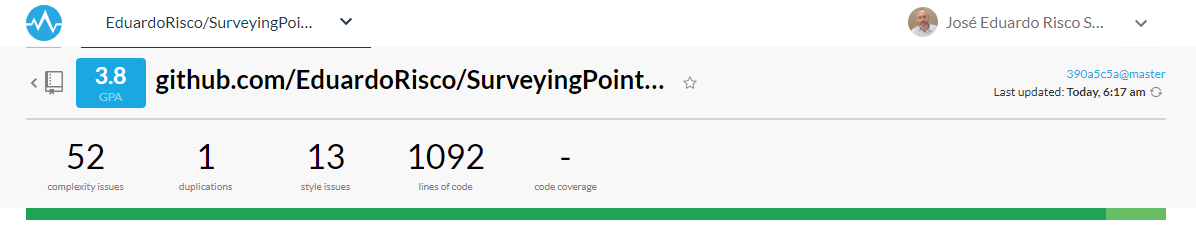
\includegraphics[width=1\textwidth]{CB_1}
	\caption{Resultado del 1º análisis con \emph{Codebeat}.}
	\label{fig:CB_1}
\end{figure}

Sobre un total de 1.092 líneas de código (estás solo son las  líneas implementadas en la aplicación, no se tienen en cuenta las librerías externas utilizadas de \emph{JavaScript} o \emph{CSS}, que se han excluido del análisis en el archivo \texttt{.codebeatignore)}, se ha obtenido una puntuación de 3,8 sobre 4. Es una puntuación bastante buena que indica un correcto desarrollo del código.

\emph{Codebeat} nos informa de la existencia de tres puntos críticos en el código que vemos a continuación:

\begin{figure}[!h]
	\centering
	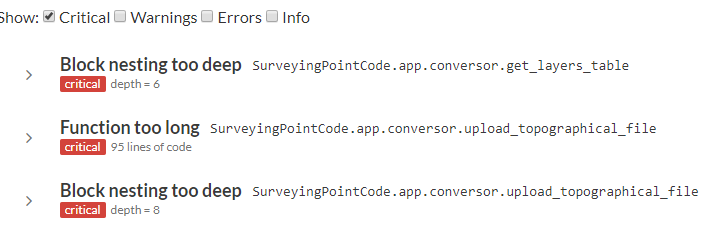
\includegraphics[width=1\textwidth]{CB_2}
	\caption{Puntos críticos del código.}
	\label{fig:CB_2}
\end{figure}

localizados en dos funciones:
\begin{enumerate}

\item \texttt{upload\_topographical\_file()}: En esta función \emph{Codebeat} indica que la profundidad máxima que alcanzan los bucles y condicionales es de 8, y también, que la longitud de la función es de 95 líneas. Como en el resto del código, se podía haber dividido está función en otras más pequeñas, pero en esté caso se ha primado leer una sola ver los datos y crear todos los elementos interpretados en un solo recorrido.

\item \texttt{get\_layer\_table()}: En esta función \emph{Codebeat} indica que la profundidad máxima que alcanzan los bucles y condicionales es de 8. Como en el caso anterior, se podía haber dividido está función en otras más pequeñas, pero en esté caso se ha primado también  leer una sola ver los datos y crear todos los elementos interpretados en un solo recorrido.
\end{enumerate}

Se han realizado cambios en el código para intentar reducir estos puntos críticos, quedando en análisis finalmente:

\begin{figure}[!h]
	\centering
	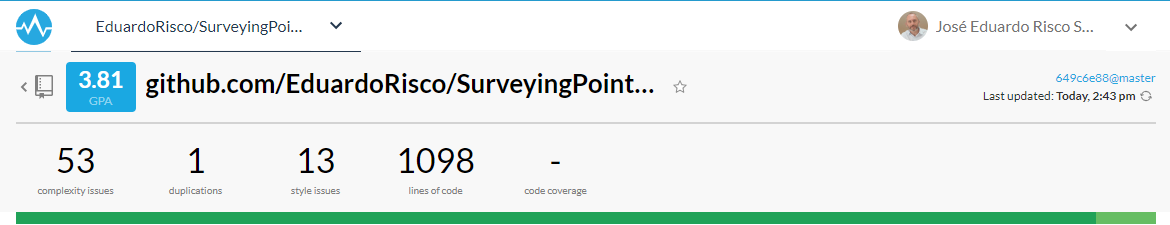
\includegraphics[width=1\textwidth]{CB_3}
	\caption{Resultado del 2º análisis con \emph{Codebeat}.}
	\label{fig:CB_3}
\end{figure}

La puntuación final se ha mejorado poco, 0.01, pero se han logrado evitar dos puntos críticos:

\begin{figure}[!h]
	\centering
	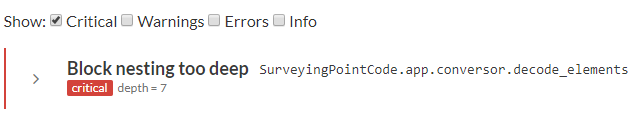
\includegraphics[width=1\textwidth]{CB_4}
	\caption{Reducción de 2 puntos críticos del código.}
	\label{fig:CB_4}
\end{figure}

El resultado del análisis de la calidad del código es muy bueno, se ha puesto mucho interés durante el proyecto en desarrollar un código de calidad que sea fácilmente entendible, extensible y reusable.

Por último, hay que indicar que el informe con la calidad del código se encuentra disponible en el siguiente enlace:\\
 \url{https://codebeat.co/projects/github-com-eduardorisco-surveyingpointcode-master}
 
\capitulo{6}{Trabajos relacionados}

Este apartado sería parecido a un estado del arte de una tesis o tesina. En un trabajo final grado no parece obligada su presencia, aunque se puede dejar a juicio del tutor el incluir un pequeño resumen comentado de los trabajos y proyectos ya realizados en el campo del proyecto en curso. 

\capitulo{7}{Conclusiones y líneas de trabajo futuras}

En este apartado se exponen las conclusiones derivadas del trabajo, así como
las posibles líneas de trabajo futuras por las que se puede dar continuidad al
proyecto y mejorar el producto.

\section{Conclusiones}

Una vez finalizado el proyecto, se han obtenido las siguientes conclusiones:

\begin{itemize}
\item El objetivo principal del proyecto se ha cumplido. Se ha desarrollado una aplicación que mediante un sistema de codificación de puntos aquí definida, consigue \textbf{automatizar el proceso de delineación} de un levantamiento topográfico. Convirtiendo un archivo de campo a un archivo DXF. Permitiendo al usuario poder subir una configuración personalizada y un archivo con símbolos. La aplicación también permite generar el archivo DXF en varias versiones de CAD. 

\item Se ha conseguido también, que el tipo de codificación definida, permita \textbf{mejorar el rendimiento en campo} a la hora de realizar el levantamiento topográfico. Mejoramos el rendimiento, al no tener que medir las líneas de forma consecutiva, creando cuadrados con solo dos puntos o rectángulos con tres puntos,etc, todo esto debido a la interpretación de la codificación.

\item No menos importante es resaltar que el usuario puede generar un plano en DXF, sin necesidad de tener conocimientos en programas de CAD.

\item En el proyecto se han utilizado los conocimientos adquiridos cursando el grado, en algunos casos requiriendo un conocimiento más profundo de estos. En otras disciplinas o tecnologías, como el desarrollo desarrollo de aplicaciones Web y el uso de Docker, se ha partido prácticamente de cero.
El tiempo dedicado a la investigación, seguro resultará una buena base para el futuro.

\item Se ha realizado este trabajo como si fuera un proyecto real,
utilizando la  metodología ágil \textbf{Scrum} en la gestión, comprobando las ventajas de su uso. Este tipo de metodología, ayuda a tener una visión más realista en cuanto a los objetivos que se desean conseguir, la planificación que se hace en los \emph{sprints} definiendo tareas alcanzables, hace que no pierdas el rumbo y vayas consiguiendo los objetivos paso a paso, ganando confianza cada vez que consigues los objetivos. 
\end{itemize}

Por último señalar, que la aplicación ha sido probada en un entorno real de trabajo por profesionales de la topografía. Se ha utilizado en campo el sistema de codificación aquí definido y posteriormente, la aplicación para generar el plano en DXF. La valoración ha sido muy positiva por parte de todos los que la han probado.

\section{Líneas de trabajo futuras}

Aunque este trabajo como Trabajo Fin de Grado acaba aquí, habiendo desarrollado la parte mas compleja y difícil de la aplicación, y definiendo sistema para codificar los puntos de campo, el proyecto seguirá avanzando. \emph{SurveyingPointCode} pretende que el producto final sea un plano completo, añadiendo elementos como:



\begin{itemize}
\item Pre visualizar el plano en el navegador.
\item Incluir marco en el plano.(ver Figura~\ref{fig:marco})
\item Incluir cajetín en el plano.(ver Figura~\ref{fig:cajetin})
\item Incluir leyenda en el plano.(ver Figura~\ref{fig:leyenda})
\item Permitir al usuario elegir el formato del plano, A0, A1, A2, etc.
\item Permitir al usuario elegir la escala del plano, 1:1000 , 1:5000 , etc.
\item Imprimir el plano.
\item Internacionalización de la aplicación.
\item Implementar un cuadro de mandos para que el administrador de la aplicación visualice las estadísticas de uso.
\item Implementar un servicio de \emph{logs} en el servidor.
\end{itemize}

\imagen{marco}{Detalle marco de un plano}
\imagen{cajetin}{Detalle cajetín de un plano}
\imagen{leyenda}{Detalle leyenda de un plano}

En definitiva, poder generar un plano como ya hemos visto, de forma automática, profesional y sin necesidad tener conocimientos en programas de CAD.



\bibliographystyle{plain}
\bibliography{bibliografia}

\end{document}
